\documentclass[11pt]{article}

\usepackage{fullpage}
\usepackage{url}
\usepackage{todonotes}
\usepackage{amsmath}
\usepackage{amsthm}
\usepackage{amsfonts}
\usepackage{amssymb}
\usepackage[utf8]{inputenc}
\usepackage{soul}
\usepackage{multicol}
\usepackage[numbers]{natbib}
\usepackage[ruled, vlined, linesnumbered]{algorithm2e}
\usepackage{placeins}
\usepackage{hyperref}
\usepackage{caption}
\usepackage{subcaption}

% Theorem and Math macros borrowed from 
% CS Professor Matt Anderson
% ------- Theorem and related environments --------
\newtheorem{theorem}{Theorem}
\newtheorem{conjecture}{Conjecture}
\newtheorem{proposition}{Proposition}
\newtheorem{claim}{Claim}
\newtheorem{lemma}{Lemma}
\newtheorem{corollary}{Corollary}
\newtheorem{definition}{Definition} 
\newtheorem{problem}{Problem}
\newtheorem{observation}{Observation}
\newtheorem{fact}{Fact}

\newcommand{\NN}{\mathcal{N}} % Natural Numbers
\newcommand{\RR}{\mathcal{R}} % Real Numbers
\newcommand{\ZZ}{\mathcal{Z}} % Integers
\newcommand{\QQ}{\mathcal{Q}} % Rational Numbers

\newcommand{\set}[1]{\ensuremath{\{{#1}\}}} % Set
\newcommand{\bigset}[1]{\ensuremath{\left\{{#1}\right\}}}
\newcommand{\condset}[2]{\ensuremath{\set{{#1}\;|\;{#2}}}} % Conditional set
\newcommand{\nin}{\not\in}
\newcommand{\cross}{\times} % Cartesian product
\newcommand{\ssn}{\subsetneq} % Proper subset
\newcommand{\sse}{\subseteq} % Subset

\DontPrintSemicolon
\newcommand{\spa}{\rightsquigarrow}
\newcommand{\td}{\todo[inline]}

\begin{document}

\title{Heuristic Algorithms for Bike Route Generation}
\author{Aidan Pieper}
\maketitle

\begin{abstract}
   \td{Write Abstract!}
\end{abstract}

\section{Introduction}
Cycling is a popular and diverse activity enjoyed by millions of people all over the world. To some, cycling is a means of commuting to work while to others it is a recreational sport.  The quality of cycling infrastructure varies across the globe. In countries like Belgium and the Netherlands where cycling is a popular recreational sport, there are vast networks of bicycle-friendly secondary roads \cite{souffriau2011planning}. However, many places do not have this same level of cycling infrastructure so bike riders must share highways with other road vehicles.


When determining routes to bike, recreational cyclists consider different factors such as route distance, elevation gain (i.e. hills), maximum percent gradient (i.e. road steepness), and how pleasant a road is to travel by bike. Designing a route that fits all user-specified criteria is a difficult task.  Moreover, there are no set criteria which determine a ``preferable" cycling route. The desirability of a given route is based on the rider's personal preferences, goals, and fitness. This research explores different algorithms to generate cycling routes for recreational road cyclists.


Most bike rides begin and end in the same location. Using this assumption, this research focuses specifically on generating preferable \emph{circular} cycling routes. For example, a cyclist may want a 15-mile route which starts and ends at their home.
    

\subsection{Motivations}
Traditional route planning problems focus mainly on finding the shortest path in a graph optimizing for either distance or time. Currently, there exists numerous route planning tools (e.g. \href{https://www.strava.com/routes/new}{Strava.com}, \href{https://www.mapmyride.com}{mapmyride.com}, and \href{https://ridewithgps.com}{ridewithgps.com}) which allow users to add points on a map and generate a route between such destinations.

However, route planning for recreational cyclists poses a fundamentally different problem than traditional route planning problems because the shortest route is not necessarily the 	preferable cycling route. Recreational cyclists generally prefer longer, more scenic, and less trafficked routes as the goal of the activity is recreation not transportation. 

%\td{Add info about traveling cyclists}


\subsection{Related work} \label{relatedwork}
In the literature, planning preferable cycling routes is modeled as an instance of the Arc Orienteering Problem (AOP), a variant of the Orienteering Problem (OP) \cite{souffriau2011planning}. First introduced in 1987 by \citeauthor{golden1987orienteering}, the classical OP is a combination of node selection and determining shortest paths between nodes in a graph \cite{golden1987orienteering}. Therefore, the OP is a hybrid between two classical combinatorial problems, the Knapsack Problem and the Traveling Salesman Problem (The OP may sometimes be referred to as the \emph{Selective} Traveling Salesman Problem \cite{laporte1990selective}). In the classical OP, each node in the graph is assigned a non-negative score and a non-negative cost. Given a starting node, a destination node, and some maximum cost budget, the objective is to determine a path which starts at the starting node, visits some subset of the graph nodes, and ends at the destination node \cite{gunawan2016orienteering}. In addition, the solution path must both maximize the total collected score (accrued from visiting a node) and keep the total collected cost under the specified budget.

The AOP is the arc variant of the OP where each arc (i.e. graph edge) is given a score and a cost. In the AOP, scores and costs are accrued from visiting an arc instead of a node. For example, Figure \ref{fig:aop-example} shows an undirected AOP instance where $S$ is the start node, $D$ is the destination node, the budget is 10, and every edge is labeled (score, cost). The shortest path is $S \rightarrow (10,3) \rightarrow (5,5) \rightarrow D$ which has a cost of 8 and a score of 15. However, for the specified budget, $S \rightarrow (20,1) \rightarrow (3,2) \rightarrow (2,2) \rightarrow (5,5) \rightarrow D$ is the optimal solution with a score of 30 and a cost of 10. Note that the optimal solution is clearly not the shortest path but rather the path with the maximal score constrained by the cost budget.

Previous research has shown that both the OP and the AOP are NP-Hard problems for directed and undirected graphs. Therefore, no algorithms are known to exist to \emph{optimally} solve the AOP or OP in polynomial time. While there is considerable research into the OP and its variants, there is less research into the AOP. \citeauthor{gunawan2016orienteering} provide an exhaustive survey of the OP and its variants, but the AOP is clearly over shadowed by other OP variants in the literature \cite{gunawan2016orienteering}.

\begin{figure}[h]
\begin{center}
    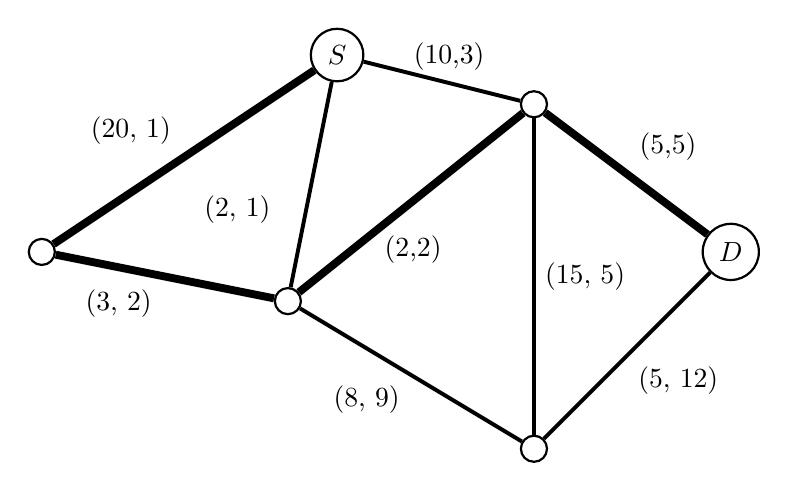
\begin{tikzpicture}[auto,x=1.25cm, y=1.25cm,line width=0.5mm]
    
        \begin{scope}[every node/.style={circle,thick,draw}]
        \node(1) at (0,0) {$S$};
        \node(2) at (2, -0.5) {};
        \node(3) at (4, -2) {$D$};
        \node(4) at (2, -4) {};
        \node(5) at (-0.5, -2.5) {};
        \node(6) at (-3, -2) {};
        \end{scope}
        
        \draw (1) -- node[xshift=-0.5cm] {(10,3)} (2);
        \draw[line width=1mm]  (2) -- node {(5,5)} (3);
        \draw (3) -- node {(5, 12)} (4);
        \draw (2) -- node {(15, 5)} (4);
        \draw[line width=1mm] (2) -- node[yshift=-0.25cm, xshift=-0.5cm] {(2,2)}(5);
        \draw (4) -- node {(8, 9)}(5);
        \draw[line width=1mm] (5) -- node {(3, 2)} (6);
        \draw[line width=1mm] (6) -- node[] {(20, 1)} (1);
        \draw (1) -- node [xshift=-1.5cm]{(2, 1)} (5);
    
    \end{tikzpicture}
\end{center}
\caption{Undirected AOP instance with start node $S$ and destination $D$. Arc label is (score, cost). Bold path is optimal for a budget of 10 (score = 30, cost = 10). Note that the bold path is not the shortest path.\label{fig:aop-example}}
\end{figure}

 
\citeauthor{gavalas2015approximation} show approximation algorithms for the AOP in both directed and undirected graphs. A polylogarithmic approximation algorithm is given for directed graphs while a $(6 + \epsilon + o(1))$-approximation algorithm is given for undirected graphs \cite{gavalas2015approximation}. Moreover, they show a reduction from the AOP to the OP. Using an existing OP approximation algorithm by \citeauthor{nagarajan2011directed}, this reduction yields a $O(\frac{log^2m}{loglogm})$-approximation algorithm for solving the AOP in directed graphs where $m$ is the number of edges \cite{gavalas2015approximation}.

Both \citeauthor{souffriau2011planning} and \citeauthor{verbeeck2014extension} study the AOP in the context of cycle trip planning. \citeauthor{souffriau2011planning} provide an integer programming mathematical model for the AOP and a heuristic algorithm for solving AOP instances to near optimality in a few seconds. To evaluate performance of their algorithm, the authors test their algorithm against a road network of bike-friendly roads in East Flanders \cite{souffriau2011planning}. The East Flanders' bicycle road network covers 5 regions and is comprised of 989 nodes with 2963 arcs for a total of 3585 km (2227 mi) of road. This model for the AOP, tailored towards recreational cycling routes, requires that each node and edge is visited at most once by the solution path and prevents sub-tours. \citeauthor{souffriau2011planning} present an algorithm based on a greedy randomized adaptive search procedure method \cite{souffriau2011planning}.

On the other hand, \citeauthor{verbeeck2014extension} consider the cycle trip planning problem in a directed graph where the goal is to maximize the total collected score which represents the attractiveness of the travelled arcs. In this model, the preferred length of the route is replaced with an upper and lower bound of the total trip distance. Unlike, \citeauthor{souffriau2011planning}, this model allows the route to visit the same vertex multiple times but visiting the same arc twice is not allowed. A two-way road can be travelled exactly once in each direction since it is modeled by two separate edges in the directed graph. The authors propose two heuristic algorithms for solving cycle trip planning instances; A branch-and-cut algorithm and an iterated local search algorithm \cite{verbeeck2014extension}. Both algorithms were evaluated by running them on the East Flanders road network dataset provided by \citeauthor{souffriau2011planning}

Similarly, research by \citeauthor{bergman2015optimization} defines the ``Circular Cycle Tour Problem" as a cycle trip planning problem where the start and end location are the same. Like other cycle routing problems, they model it as an instance of the AOP. \citeauthor{bergman2015optimization} use a popularity weighted road network graph using road popularity data from smartphone fitness tracking application \href{http://www.sports-tracker.com/}{sports-tracker.com} (i.e, the most popular roads have high positive scores) \cite{bergman2015optimization}. They present a heuristic algorithm that starts with initial random cyclic routes and iteratively improves them to find a locally optimal route.

\subsection{Modeling Preferability of Cycling Routes} \label{routefactors}
As mentioned previously, recreational cyclists consider many factors when designing a preferable cycling route. The following is a non-exhaustive list of such factors:

\begin{multicols}{2}
\begin{itemize}
    \item Route distance
    \item Route elevation gain
    \item Time
    \item Maximum percent gradient
    \item Amount of traffic
    \item Number of intersections
    \item Good cellular service
    \item Easy parking at start
    \item Availability of restrooms
    \item Availability of rest stops and food
    \item Scenery
    \item Proximity to bike shops
    \item Proximity to mass transit
    \item Limited uphill at end of ride
\end{itemize}    
\end{multicols}

Many of these factors can be modeled nearly identically. For example, distance, elevation gain, and time are all calculated by the sum of those weights over all roads in the route. On the other hand, maximum percent gradient can be seen as a ``boolean criterion." That is, a road's steepness is either under the maximum percent gradient or over, in which case the road does not satisfy this criterion. If these boolean criteria must be avoided, a simple option is to initially remove or ``prune" all roads from the graph which do not meet these criteria.

In previous research, the cost of a particular arc is usually the distance of the  road and the score is some measure of the preferability of the road (e.g. popularity). Since the AOP requires a single value for the cost and score of each arc, computing costs and scores as linear combinations of different variables is a one way to model multiple factors. For example, a particular road's cost might be a combination of its distance, its elevation gain, and the level of traffic on the road. This allows one to give certain factors more importance by weighting them more heavily in the linear combination. Furthermore, one might want to avoid certain boolean criteria instead of outlawing them entirely. For instance, one could give the presence of a dirt road a small weight in the cost of a road which means dirt roads will have slightly higher costs.

While multiple route factors are important to recreational cyclists, the focus of this research is not to model the preferability of roads. Hence, we assume that we have the necessary data to appropriately score roads for recreational cyclists. In other words, the focus of this research is on the route planning algorithm, not creating the graph (with the associated scores and costs) which represents the AOP instance.


\subsection{Research Question}
As mentioned in Section \ref{relatedwork}, existing literature models cycle trip planning as an instance of the AOP. This research follows the existing literature and focuses on implementing and improving existing AOP algorithms for cycle route planning. 

Since road networks can be quite large and because the AOP is NP-Hard, searching for the optimal route may take an unacceptable amount of time. Since we care more about finding a good route than finding the best possible route, we trade off optimality for speed. However, even AOP approximation algorithms are too slow for applications where a fast response time (on the order of milliseconds) is required \cite{lu2015arc}. Therefore, we focus on heuristic algorithms for route generation. Both \citeauthor{verbeeck2014extension} and \citeauthor{lu2015arc} propose heuristic algorithms which follow the Iterated Local Search (ILS) framework. This framework, and their respective algorithms are the focus of the following sections. Thus, our research question is as follows:

\begin{quote}
    To what extent can ILS algorithms be improved to generate better bike routes?
\end{quote}

In the following sections we refer to the the algorithm proposed by \citeauthor{verbeeck2014extension} as the \emph{VVA Algorithm} and the algorithm proposed by \citeauthor{lu2015arc} as the \emph{LS Algorithm}.


\section{Methods}

\subsection{Iterated Local Search}
Iterated Local Search (ILS) is a framework for solving optimization problems using heuristic search algorithms. A heuristic is a technique used to solve a problem quickly when exact or approximation methods are too slow. Heuristic algorithms can be thought of as ``shortcuts" in that they trade optimality and completeness for speed. Heuristics are often used in search algorithms to  determine which branch of the search to take but are not guaranteed to produce the best solution. A heuristic algorithm is commonly referred to as a heuristic.

Local Search is a heuristic method for solving optimization problems. Local Search starts with a candidate solution and moves to a ``neighbor" solution which is better than the current solution as defined by an objective function (a function which scores solutions in the search space) \cite{gendreau2010handbook}. Local Search can get stuck in local optima which are points in the search space that are better than all neighbors but are not the best possible solution.

ILS is a variant of Local Search to stop it from getting trapped in local optima. Instead of repeating random trials of the heuristic algorithm, ILS builds a sequence of locally optimal solutions generated by the heuristic which is more likely to lead to a better overall solution \cite{gendreau2010handbook}. This is done by first generating an initial solution using the search heuristic, perturbing the current solution (or changing the solution), and applying the search heuristic again on the modified solution. The perturbation and local search steps are then repeated until some condition, usually time, is met.
The following pseudocode outlines the ILS framework:

%
% Iterated Local Search definition
%
\begin{algorithm}[!h]
\caption{ILS($t$, $localsearch$, $score$)}
\KwData{$t$: a time, $localsearch$: a heuristic search function, $score$: an objective function.}
\KwResult{A solution of the $localsearch$ function.}
S $\gets$ $localsearch$(empty solution)\;
\While{$t$ seconds have not elapsed}{
    $S^* \gets$ perturb $S$\;
    $S' \gets localsearch(S^*)$\;
    \If{$score(S') > score(S)$}{
        $S \gets S'$\;
    }
}
\KwRet{S}
\end{algorithm}

Despite its simplicity, ILS can be challenging to implement efficiently because many implementation choices are left to the developer. For example, an efficient ILS implementation requires a certain level of domain specific knowledge. The main issue with ILS is that the algorithm may get ``trapped" in a local maximum over many iterations. Therefore, the modification (perturbation) step must modify the search solution enough to make progress but not too much that the search is effectively starting with a different ``random" solution upon each iteration. 

% TODO(Aidan) draw picture of ils peaks and troughs


\subsection{VVA Algorithm}
%\td{The graph $G$ is never passed in anywhere in the pseudocode??}
The local search algorithm proposed by \citeauthor{verbeeck2014extension} is a modified version of Depth First Search (Algorithm \ref{alg:dfs}). It is implemented as a recursive function which used to to find a path between two disconnected nodes in the bike route. The algorithm is allowed to ``take" an outgoing edge and add it to the current route as long as it has not been traversed before and the shortest path from the end of the traversed arc to the destination is less than the remaining distance after taking the arc (Line \ref{alg:dfs:feasability}). In other words, it must be \emph{feasible} to get from the end of the chosen arc to the desired destination after traversing the arc. Since this requires many shortest path computations, the VVA algorithm assumes that all-pairs shortest path have been pre-computed before the ILS runs. In Algorithm \ref{alg:dfs}, the function $shortestPath(v_1, v_2)$ would return the pre-computed shortest path. In addition, the $maxDepth$ parameter is used to restrict the depth of the search and reduce the search space (Line \ref{alg:dfs:depth}).

\begin{algorithm}[!h]
    \caption{DFS($route$, $s$, $d$, $dist$, $minProfit$, $maxDepth$)\label{alg:dfs}}
    \KwData{$route$: a temporary solution, $s$: the start node of the path, $d$: the end node of the path, $dist$: the maximum cost of the route, $minProfit$: the minimum score of the route, $maxDepth$: the maximum number of edges allowed in the solution, $shortestPath(v_1, v_2)$: a function which returns the shortest distance between two nodes of the graph, and $edges(v_1)$: a function which returns all edges of a node. 
        }
    \KwResult{A boolean which denotes whether a path was found. If true, the solution is contained inside of $route$.}
    \If{$maxDepth < 0$}{\label{alg:dfs:depth}
        \KwRet{false}\;
    }
    \For{$arc \in edges(s)$}{ \label{alg:dfs:for}
        \If{$arc \nin route$ and $arc.cost + shortestPath(arc.end, d) < dist$}{\label{alg:dfs:feasability}
            Add $arc$ to $route$\;
            \uIf{$arc.end = d$ and $route.score > minProfit$}{\label{alg:dfs:end}
                \KwRet{true}\;
            } \ElseIf{DFS(route, arc.end, d, dist - arc.cost, minProfit, maxDepth - 1)}{\label{alg:dfs:recurse}
                \KwRet{true}\;
            }
            Remove $arc$ from $route$\;
        }\label{alg:dfs:endfor}
    }
\KwRet{false}\;
\end{algorithm} 

Using this DFS algorithm as the local search heuristic \citeauthor{verbeeck2014extension}, apply the ILS framework to create a bike route planning algorithm. Algorithm \ref{alg:ils-ver} first generates an initial route using the DFS heuristic and stores the path in the variable $route$ (Line \ref{alg:ilsv:init}). The ILS perturbs the solution by removing a path segment from the solution and invoking the DFS procedure to find a new solution (Lines \ref{alg:ilsv:perturb}-\ref{alg:ilsv:improve}). In the perturbation phase, the algorithm removes $R$ consecutive arcs starting at the arc at position $A$ in solution $route$. If a new path is found after removing a path segment from the solution, then the new path is merged into the current solution (Line \ref{alg:ilsv:merge}). If no new path can be found, then there is no improvement so $A$ and $R$ are both incremented by 1 (Line \ref{alg:ilsv:increment}).

%
% VVA ILS Algorithm
%
\begin{algorithm}[!h ]
    \caption{ILS-VVA($s$, $d$, $dist$, $maxDepth$, $t$) \label{alg:ils-ver}}
    \KwData{$s$: the start node of the path, $d$: the end node of the path, $dist$: the maximum distance of the path, $maxDepth$: the maximum depth allowed in the DFS, and $t$: a time.}
    \KwResult{a path.}
    
    $route \gets$ empty route\;
    \If{not DFS(route, s, d, dist, 0, maxDepth)}{\label{alg:ilsv:init}
        $route \gets$ empty route\;
    }
    $A \gets 1$, $R \gets 1$\;
    
    \While{$t$ seconds have not elapsed}{
        $temp \gets$ copy of $route$\;
        \If{$R > temp.length$}{
            $R \gets 1$\;
        }
        
        \If{$A + R > temp.length -1$}{
            $R \gets temp.length - 1 - A$\;
        }
        
    
        Remove $R$ arcs from $temp$ starting at arc at index $A$\; \label{alg:ilsv:perturb}
        $minScore \gets$ sum of scores of removed arcs from $temp$\;
        $s^* \gets$ starting node of first arc removed\;
        $d^* \gets$ ending node of last arc removed\;
        $new \gets$ empty route\;
        
        \If{DFS(new, $s^*$, $d^*$, dist - temp.dist, minScore, maxDepth)}{\label{alg:ilsv:improve}
            Merge $new$ into $temp$ at index $A$\; \label{alg:ilsv:merge}
            $route \gets temp$\;
            $A \gets 1$, $R \gets 1$\;
        } \Else {
            $A \gets A + 1$, $R \gets R + 1$\; \label{alg:ilsv:increment}
        }
    
    }
    
    \KwRet{route}        
\end{algorithm}

%\td{Move this to evaluation?}
The main drawback of the VVA algorithm is that the ILS has slow iteration because it is performing DFS on every iteration.  Moreover, it requires many shortest paths to be precomputed before the algorithm can run. This can be infeasible on large real-world  mapping datasets. Since the algorithm assumes all pairs shortest-path pre-computated, the feasibility checking used by the search is $O(degree^{maxDepth})$ where $degree$ is the average degree of nodes in the road network and $maxDepth$ is the maximum depth allowed in the DFS.

\subsection{LS Algorithm}
At a high level, the ILS algorithm proposed by \citeauthor{lu2015arc} restricts the search space by using spatial indices to prune arcs from the search. Instead of relying on pre-computed shortest paths, the LS algorithm uses online shortest path computations but does less feasibility checking due to the spatial restrictions (See Section \ref{sec:pruning} for more information).

\subsubsection{Attractive Arcs}
\citeauthor{lu2015arc} define their solution route in terms of ``attractive arcs" which are arcs with a positive score (i.e. $arc.score > 0$). A path from node $v_1$ to $v_2$ is a series of attractive arcs $(a_1, a_2, \ldots, a_n)$ which starts with $a_1$, ends with $a_n$ and is denoted by, $(v_1 \spa a_1 \spa a_2 \spa \ldots \spa a_n \spa v_2)$. The symbol $\spa$ denotes the shortest path in the graph between two nodes or arcs. The path between two adjacent attractive arcs ($a_i \spa  a_{i+1}$) is known as the ``blank path segment" and is the shortest path from the end vertex of $a_i$ to the start vertex of $a_{i+1}$. These vertices are respectively denoted $l_i.start$ and $l_i.end$. Given an attractive arc $a_i$ from a solution path, $a_i.pre$ refers to the previous attractive arc ($a_{i-1}$) and $a_i.post$ refers to the next attractive arc in the path ($a_{i+1}$). The total cost of a path is the sum of all costs of all the arcs in the path, including the arcs in the blank path segments. The score of a path is defined similarly. To build a solution, the LS algorithm connects many attractive arcs together using shortest path blank path segments.

\subsubsection{Candidate Arc Set}
Every arc $a$ in the solution $S$ is associated with a set of candidate attractive arcs. 
%
% Definition of Candidate Arc Set
%
\begin{definition}[\cite{lu2015arc}]
    Let $a \in S$ be an arc in the solution $S$ whose distance budget is $B$. Then the Candidate Arc Set (CAS) of $a$, denoted by $a.CAS$ is the set of arcs who have a positive score and can feasibly update (replace) $a$ in $S$, i.e. $\forall a_c \in a.CAS, a_c.score > 0$ and $(a.pre \spa a_c \spa a.post).cost < B - S.cost + (a.pre \spa a \spa a.post)$.
\end{definition}

\citeauthor{lu2015arc} show that candidate arc sets have the following inherited property. This allows the search space to be reduced when computing some CASs since the parent CAS can be restricted.
\begin{lemma}[\cite{lu2015arc}] Let $a$ be an arc. Given $a.CAS$, $\forall a_c \in a.CAS, a_c.CAS \sse a.CAS$.
\end{lemma}

To chose which candidate arcs to add to the solution, \citeauthor{lu2015arc} propose a criteria called ``Quality Ratio" which is defined for an arc $a_c$ from the candidate arc set $a.CAS$ of a solution arc $a$. The intuition is that arcs with higher value and lower cost will be more likely to improve the solution. In order to determine which arcs to remove from the solution in the ILS perturbation, they propose a criteria called ``Improve Potential". The intuition is that solution arcs with lower scores and more valuable nearby arcs are more likely to improve the solution.

Algorithm \ref{alg:ils-lu-compcas} performs the feasibility checking to generate a set of candidate arcs which can be used to connect the start node $v_1$ to the destination node $v_2$. The algorithm takes in a set of possible arcs, iterates over each one, and adds the arc to the current CAS only if its score is positive and the distance of the path from $v_1$ to $a$ to $v_2$ is within the specified budget (Lines \ref{alg:ils-lu-compcas-for}-\ref{alg:ils-lu-compcas-add}). In addition, the Quality Ratio is calculated for the specified arc in the CAS (Line \ref{alg:ils-lu-compcas-qr}). If the CAS, $A$, passed into the algorithm is non-empty, then it can use the ``CAS inherit" property and filter out arcs whose paths are within the new specified budget. If the CAS passed in is non-empty, then the algorithm will iterate over all arcs in the graph to find the ones which can be feasibly inserted (Lines \ref{alg:ils-lu-compcas-if}-\ref{alg:ils-lu-compcas-ifend}).


%
% Compute Candidate Arc Set algorithm
%
\begin{algorithm}[!h]
    \caption{computeCAS($G$, $A$, $v_1$, $v_2$, $dist$) \label{alg:ils-lu-compcas}}
    \KwData{$G$: the road network graph, $A$: a candidate arc set, $v_1$: start node, $v_2$: destination node, $dist$: allowable budget.}
    \KwResult{A set of candidate arcs.} 
    $CAS \gets \text{empty set}$\;
    \If{$A$ is empty}{ \label{alg:ils-lu-compcas-if}
    $A \gets$ all arcs from $G$\; \label{alg:ils-lu-compcas-ifend}
    }
    \For{$a \in A$}{\label{alg:ils-lu-compcas-for}
        \If(\tcp*[h]{Feasibility checking}){$a.score > 0$ and $(v_1 \spa a \spa v_2).cost \leq dist)$}{
            $a.qr = QualityRatio(v_1, v_2, a)$\; \label{alg:ils-lu-compcas-qr}
            add $a$ to CAS\; \label{alg:ils-lu-compcas-add}
        }
    }
    \KwRet{CAS}
\end{algorithm}


%
% Update Candidate Arc Set algorithm
%
\begin{algorithm}[!h]
    \caption{updateCAS($A$, $a$, $v_1$, $v_2$, $newDist$, $oldDist$) \label{alg:ils-lu-updatecas}}
    \KwData{$A$: set of all arcs in the graph, $a$: arc whose CAS needs to be updated, $v_1$: node in current path before $a$, $v_2:$ node in current path after $a$, }
    \KwResult{An updated set of candidate arcs}
    $CAS \gets a.CAS$\;
    \If(\tcp*[h]{Restrict CAS using inherit property}){$newDist < oldDist$}{\label{alg:ils-lu-updatecas-less}
        \For{$e \in a.CAS$}{
            \If{$(v_1 \spa e \spa v_2).cost > newDist$}{
                remove $e$ from $CAS$\; \label{alg:ils-lu-updatecas-lessend}
            }
        }
    } \ElseIf(\tcp*[h]{Expand CAS by checking all edges from graph}) {$newDist > oldDist$}{ \label{alg:ils-lu-updatecas-more}
        \For{$e \in A$}{
            \If{$e \nin CAS$ and $e.score > 0$ and $(v_1 \spa e \spa v_2).cost \leq newDist$}{
                add $e$ to $CAS$\; \label{alg:ils-lu-updatecas-moreend}
            }
        }
    }
    \KwRet{CAS}
\end{algorithm}

Algorithm \ref{alg:ils-lu-updatecas}'s job is to update the CAS for a particular arc $a$. If arcs are added to the current solution, then its distance changes as well as the remaining budget. For the new arcs added, computing the respective CASs using Algorithm \ref{alg:ils-lu-compcas} suffices. However, the previous arcs in the solution need to have their CASs changed since the remaining distance (budget) is now different. Algorithm \ref{alg:ils-lu-updatecas} takes in two budget values, $newDist$ and $oldDist$. If the new budget is smaller than the old budget, there may be some arcs in our CAS whose paths are too long for the new budget. Therefore, the algorithm employs CAS inheritance and restricts the current CAS by removing the arcs which can no longer be feasibly inserted with the new budget (Lines \ref{alg:ils-lu-updatecas-less}-\ref{alg:ils-lu-updatecas-lessend}). If the new budget is larger than our old budget, then the algorithm must expand the CAS by checking the feasibility of all arcs in the graph (Lines \ref{alg:ils-lu-updatecas-more}-\ref{alg:ils-lu-updatecas-moreend}).


\subsubsection{Path Generation}
Algorithm \ref{alg:ils-lu-genpath} is the local search heuristic used by the LS algorithm (Algorithm \ref{alg:ils-lu}). Its goal is to produce a path which connects the start vertex $s$ with the destination vertex $d$ whose total cost is within the budget $dist$ and total score is greater than $minProfit$. The algorithm builds the path by choosing candidate arcs from the CAS $A$.

Algorithm \ref{alg:ils-lu-genpath} first instantiates a fake arc starting and ending at the specified endpoints with a cost and score of 0 (Line \ref{alg:ils-lu-genpath-fake}). This fake arc is used to instantiate the solution to return, $route$ (Line \ref{alg:ils-lu-genpath-init}). It then obtains a set of arcs to insert by filtering the CAS $A$ by choosing arcs whose quality ratio is higher than the average (Line \ref{alg:ils-lu-genpath-arcs}). While there are still possible arcs left to insert and the path has budget left, arcs are continuously removed from the CAS and inserted into the current solution $route$ (Lines \ref{alg:ils-lu-genpath-while}-\ref{alg:ils-lu-genpath-endwhile}). The algorithm inserts these candidate arcs into the path using a greedy approach. It chooses the closest blank path segment in the solution to insert the arc into the path (Lines \ref{alg:ils-lu-genpath-blank}-\ref{alg:ils-lu-genpath-blankend}).


%
% Generate Path algorithm
%
\begin{algorithm}[!h]
    \caption{generatePath($s$, $d$, $dist$, $minProfit$, $A$) \label{alg:ils-lu-genpath}}
    \KwData{$s$: a start node of the path, $d$: the end node of the path, $dist$: the path's budget, $minProfit$: minimum score of the path, $A$: candidate arc set to choose arcs from.}
    \KwResult{a path which fits the specified criteria.} 
    
    $a_f \gets (s, d, 0, 0)$ \tcp*[h]{Arc with endpoints s \& d with cost \& score of 0}\label{alg:ils-lu-genpath-fake}\;
    $route \gets \set{a_f}$\label{alg:ils-lu-genpath-init}\;
    
    $arcs \gets$ all arcs from $A$ whose quality ratio is above the average \label{alg:ils-lu-genpath-arcs}\;
    \While {$arcs$ is not empty and $route.cost < dist$}{ \label{alg:ils-lu-genpath-while}
        $e \gets$ remove random arc from $arcs$\; 
        $l \gets$ null blank path segment \label{alg:ils-lu-genpath-blank}\;
        $minDist \gets 0$\;
        
        \For{$l_i \in$ blank path segments of $route$}{
            $dist \gets (l_i.start \spa e \spa l_i.end).cost$\;
            \If{$dist < minDist$}{
                $l \gets l_i$\;
                $minDist \gets dist$ \label{alg:ils-lu-genpath-blankend}\;
            
            }
        }
        
        $path \gets (l.start \spa e \spa l.end)$
        
        \If(\tcp*[h]{Our path can feasibly replace $l$}){$path.cost \leq dist - route.cost + l.cost$}{
            insert $path$ into $route$ at blank path segment $l$\label{alg:ils-lu-genpath-endwhile}\;
        }
    }
    
    \If{$route.score > minProfit$}{
        \KwRet{route}\;
    } \Else {
        \KwRet{empty route}\;
    }       
\end{algorithm}


Using the previously defined sub-procedures, \citeauthor{lu2015arc} define Algorithm \ref{alg:ils-lu}, an ILS algorithm for generating a bike route. First, the algorithm checks to see if the shortest path from the start to the destination is within the budget and if so then it runs the ILS. If not, it returns an empty solution (Lines \ref{alg:ils-lu-spcheck}-\ref{alg:ils-lu-spcheck2}). The ILS first initializes a fake arc with endpoints $s$ \& $d$ and a cost of $dist$ and a score of 0 (Line \ref{alg:ils-lu-fake}) then computes the CAS of this arc (Line \ref{alg:ils-lu-fakecas}). This arc is used to initialize the temporary solution (Line \ref{alg:ils-lu-init}).

While the time limit $t$ has not elapsed, the algorithm chooses arcs from the solution to be removed based on their improve potential, removes them from the solution, then uses generatePath to find a new path which closes the gap (Lines \ref{alg:ils-lu-while}-\ref{alg:ils-lu-ilsgenpath}). If $generatePath$ can find a path to close the gap, then it needs to update the CAS of all the arcs in the solution. For the new arcs from $generatePath$ being added to the solution, the candidate arc sets must be computed (Line \ref{alg:ils-lu-ilscompcas}). On the other hand, arcs already in the solution must have their CASs updated (Line \ref{alg:ils-lu-ilsupdatecas}) since the remaining budget will have changed by adding the new path segment. 

%
% Lu-Shahabi ILS algorithm
%
\begin{algorithm}[!h]
    \caption{ILS-LS($t$, $s$, $d$, $dist$, $G$) \label{alg:ils-lu}}
    \KwData{$t$: a time, $s$: the start node of the path, $d$: the end node of the path, $dist$: the maximum cost of the route, $G$: the graph of the road network.}
    \KwResult{a path}
    
    \If{$(s \spa d).cost > dist$}{\label{alg:ils-lu-spcheck}
        \KwRet{empty route} \label{alg:ils-lu-spcheck2}
    } \Else {
    
        $a_f \gets (s,d, dist, 0)$ \tcp*[h] Arc with endpoints s \& d with cost $dist$ and score 0 \label{alg:ils-lu-fake}\;
        $a_f.CAS \gets computeCAS(G, \set{}, s, d, dist)$ \label{alg:ils-lu-fakecas}\;
        $solution \gets \set{a_f}$ \label{alg:ils-lu-init}\;
        
        
        \While{$t$ seconds have not elapsed}{\label{alg:ils-lu-while}
            $arcs \gets$ all arcs from $solution$ whose improve potential is above the average\;
            $e \gets$ remove a random arc from $arcs$\;
            $b_1 \gets solution.cost + e.cost$ \tcp*[h]{Budget after removing e from solution}\;
            $path \gets generatePath(e.pre, e.post, b_1, e.score, e.CAS)$\label{alg:ils-lu-ilsgenpath}\;
            \If{$path$ is not empty}{
                remove $e$ from $solution$\;
                insert $path$ into $solution$ between $e.pre$ and $e.post$\;
                \For{$a \in route$}{
                    $b_2 \gets solution.cost + a.cost$ \tcp*[h]{Budget after removing a from solution}\;
                    \If{$a \in path$ or $a = e.pre$ or $a = e.post$}{
                        $a.CAS = computeCAS(G, a.CAS, a.pre, a.post, b_2)$\label{alg:ils-lu-ilscompcas}\;
                    } \Else {
                        $a.CAS = updateCAS(G, a.CAS, a.pre, a.post, b_1, b_2)$\label{alg:ils-lu-ilsupdatecas}\;
                    }
                }
            }
        }
        \KwRet{route}\;
    }
\end{algorithm}

\subsubsection{Spatial Pruning Techniques}\label{sec:pruning}
While Algorithm \ref{alg:ils-lu} relies on the ``CAS inherit" property to restrict the search space, it still has to do a lot of processing to generate the initial CAS or update CASs when the budget expands. For example, Line \ref{alg:ils-lu-fakecas} computes the CAS of the inital fake arc which requires checking the feasibility of every arc in the road network. Clearly, this is a large search space. In order to address this issue,  \citeauthor{lu2015arc} propose an ``ellipse pruning" technique to reduce the number of arcs which need to be checked.


An ellipse is a curve such that for every point on the curve, the sum of the distances to the two focal points is constant. Consider the scenario where there are two graph nodes $v_1$ and $v_2$ in which the desired path between the two has a budget of $b$. Furthermore, consider the ellipse whose focal points are the two nodes and whose sum of the distances to the two focal points is $b$ (Figure \ref{fig:ellipse}). For all points $p$ on the ellipse $(v_1 \spa p \spa v_2).cost = b$ where the shortest path is the straight line Euclidean distance. Therefore, if there is an arc $a$ which connects $v_1$ to $v_2$ and contains a point $p_o$ outside of the ellipse, we know that $a.cost > b$ since $(v_1 \spa p_o \spa v_2).cost > b$. This criteria is used to prune arcs from the search space when calculating or updating CASs.

\begin{figure}[!h]
\begin{center}
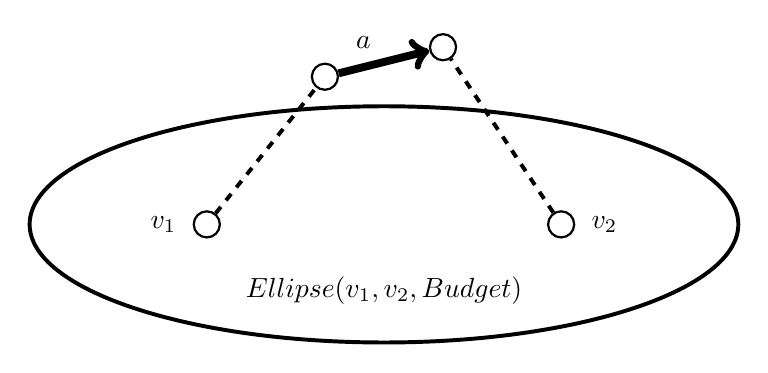
\begin{tikzpicture}[auto, x=1.5cm, y=0.75cm]
  \begin{scope}[every node/.style={circle,thick,draw}]
\node[label=left:$v_1$](1) at (0,0) {};
\node[label=right:$v_2$](2) at (3,0) {};
\node(4) at (1, 2.5) {};
\node(5) at (2, 3) {};
\end{scope}

\draw[dashed, line width=0.5mm] (1) -- (4);
\draw[dashed, line width=0.5mm] (2) -- (5);
\draw[->, line width=1mm] (4) -- node{$a$}(5);

\draw[line width=0.5mm] (1.5, 0) ellipse (4.5 cm and 1.5cm) node [below=15pt] {$Ellipse(v_1, v_2, Budget)$};
\end{tikzpicture}
\end{center}
\caption{Illustration of \citeauthor{lu2015arc}'s ellipse pruning technique. The goal is to connect $v_1$ to $v_2$ with a path of budget $b$. The arc $a$ is excluded from the search since it contains a point outside of the ellipse and is infeasible. \cite{lu2015arc}.}
\label{fig:ellipse}
\end{figure}



\section{ILS Implementation}

\subsection{OpenStreetMap}
We implement the VVA and LS algorithms and evaluate them on real world road networks. The crowd-sourced open mapping dataset \emph{OpenStreetMap} (OSM) is the natural choice for our data set. As an organization, OSM  provides a free mapping dataset for the entire planet (a full world map is around 56GB!) \cite{osm}. However, the OSM map format is an XML-based schema which is not trivially translatable into a road network graph. Luckily, in addition to open data, OSM includes a collection of open source software which interface with the data. Because the goal of this research is not to translate raw OSM data into a usable graph representation, we need software that already has this parsing capability in order to implement both ILS algorithms.

It should be noted that since OSM is a crowdsourced dataset, its level of accuracy varies across the world. This is the main drawback to using OSM. Additionally, some OSM roads (known as ``ways" in OSM parlance) contain metadata used to help bicycle routing but it is not guaranteed to be available. This bicycle routing hint is a value which is used to express the desirability of the road in the following format:  
\begin{table}[h]
\begin{center}
    \begin{tabular}{|l|p{0.75\linewidth}|}
        \hline
        \textbf{Score} & \textbf{Meaning} \\
        \hline
        -3 & ``Avoid at all cost" \\
        \hline
        -2 & ``Only use to reach your destination, not well suited" \\
        \hline
        -1 & ``Better take another way" \\
        \hline
        0 & ``As well as other ways around." \\
        \hline
        1 & ``Prefer" \\
        \hline
        2 & ``Very nice way to cycle" \\
        \hline
        3 & ``This way is so nice, it pays out to make a detour also if this means taking many unsuitable ways to get here." \\
        \hline
    \end{tabular}
\end{center}
\caption{OSM bicycle hints. Taken directly from the OSM wiki.}
\end{table}
However, the OSM wiki notes that these values ```should not be used where other attributes are considered adequate description" \cite{osm}.

\subsection{GraphHopper}
We use GraphHopper as the starting point for our research. GraphHopper is an open source routing engine written in Java which can download and parse raw OSM data into a usable graph representation \cite{graphhopper}. On top of data parsing, GraphHopper provides a web server and webpage front-end which are useful for visualizing and running routing algorithms (Figure \ref{tab:graphhopper-frontend}). Internally, GraphHopper has a number of built-in pathfinding algorithms including A* and Dijkstra which can be used for routing. These algorithm implementations provide a good template for implementing other routing algorithms with GraphHopper. 

\begin{figure}[h]
    \begin{center}
        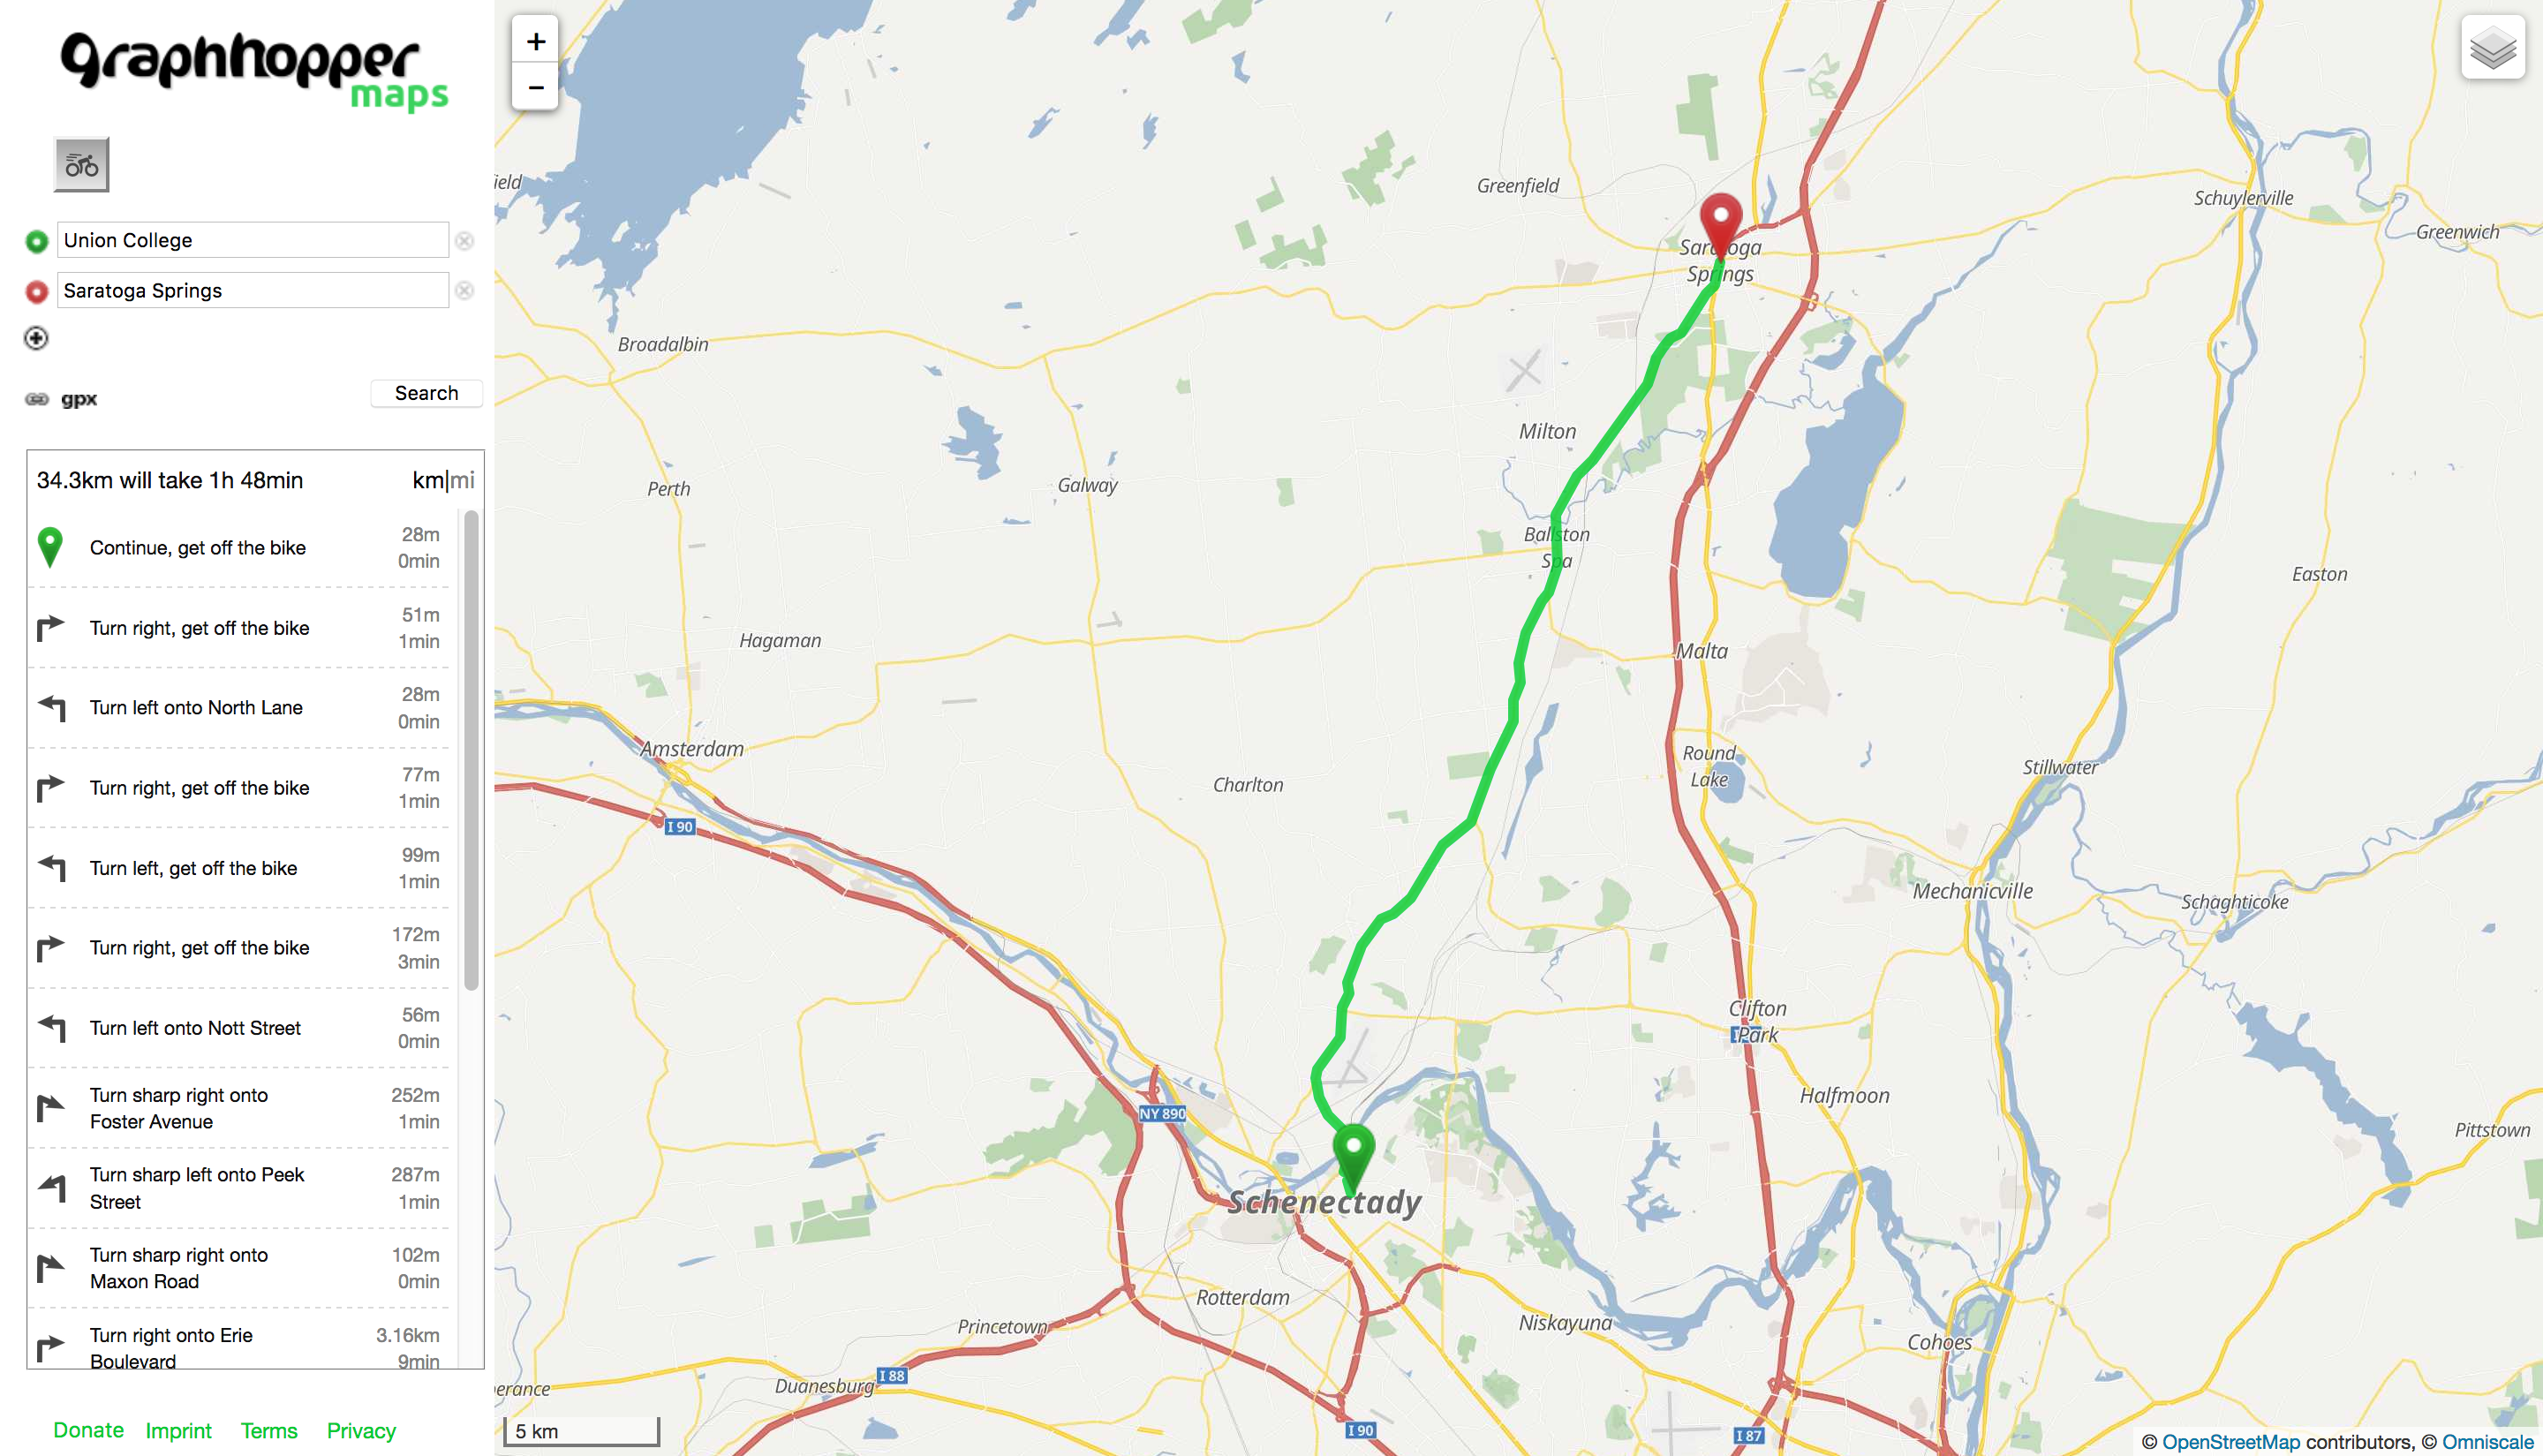
\includegraphics[width=\textwidth]{figs/graphhopper}
    \end{center}
    \caption{GraphHopper web frontend. This is OpenStreetMap data overlaid with the shortest path from Union College to Saratoga Springs.}
    \label{tab:graphhopper-frontend}
\end{figure}

Additionally, GraphHopper supports multiple ``routing profiles" which modify the weights of roads based on a particular vehicle (e.g. car, bike, walking). This is used to give preference to certain roads that are more suited for a particular vehicle. GraphHopper's default bike routing profile contains code for giving the normalized ``priority" value of a road. A normalized priority value is one of the 7 values contained in Table \ref{tab:graphhopper-frontend} normalized to a 0 to 1 scale. When determining the priority of a road, this routing profile also considers other road metadata such as road speed and road surface. We use this normalized priority value calculated by graphhopper as our road scoring mechanism. A road's cost is simply its distance in meters.


\subsubsection{Contraction Hierarchies}
GraphHopper supports a special type of graph preprocessing called contraction hierarchies \cite{graphhopper}. The goal of contraction hierarchies is to preprocess the graph such that subsequent shortest path queries can be done more quickly but still provably optimal. This is done by ordering nodes by some importance value and then iteratively contracting the least important node. Contracting a node $v$ means replacing shortest paths through $v$ with new shortcut edges \cite{geisberger2008contraction}. A faster shortest path search can be obtained by running a bidirectional shortest-path search making sure that the forward direction only traverses edges going to more important nodes and the backward direction only traverses edges coming from more important nodes.

When running the GraphHopper server for the first time, the engine processes the raw OSM data into a graph and builds contraction hierarchies for each of the enabled routing profiles. This contraction step may take many minutes depending on the size of the graph. We use GraphHopper's built-in contraction hierarchy based shortest path algorithm (Bidirectional Dijkstra's algorithm) for calculating shortest paths in both our VVA implementation LS implementation.

\subsection{VVA Implementation}
Our Java implementation of the VVA algorithm differs very little from the pseudocode proposed by \citeauthor{verbeeck2014extension} Our implementation does not have a set of starting locations nor does it retain the four best initial solutions. Rather, the starting location is fixed and only the single highest scoring solution is retained between iterations. Our local search heuristic is still a recursive DFS with a maximum depth parameter and arc feasibility checking.

Another difference in our implementation is how we check arc feasibility. Instead of precomputing all-pairs shortest path, we use GraphHopper's built in contraction hierarchies and do an online shortest-path computation. It should be noted that this is slower than assuming all shortest paths have been computed and using a lookup table. However, this requires far less computation before the algorithm runs. In addition, we can leverage GraphHopper's fast and correctly implemented shortest-path algorithms without writing our own pre-processing code. Since we are routing on a contraction hierarchy graph, we need to make sure to ignore the special ``shortcut" edges added in the contraction phase.

Lastly, recall that our road scoring mechanism is GraphHopper's normalized priority value and road costs are distances in meters.

\begin{figure}
    \begin{center}
        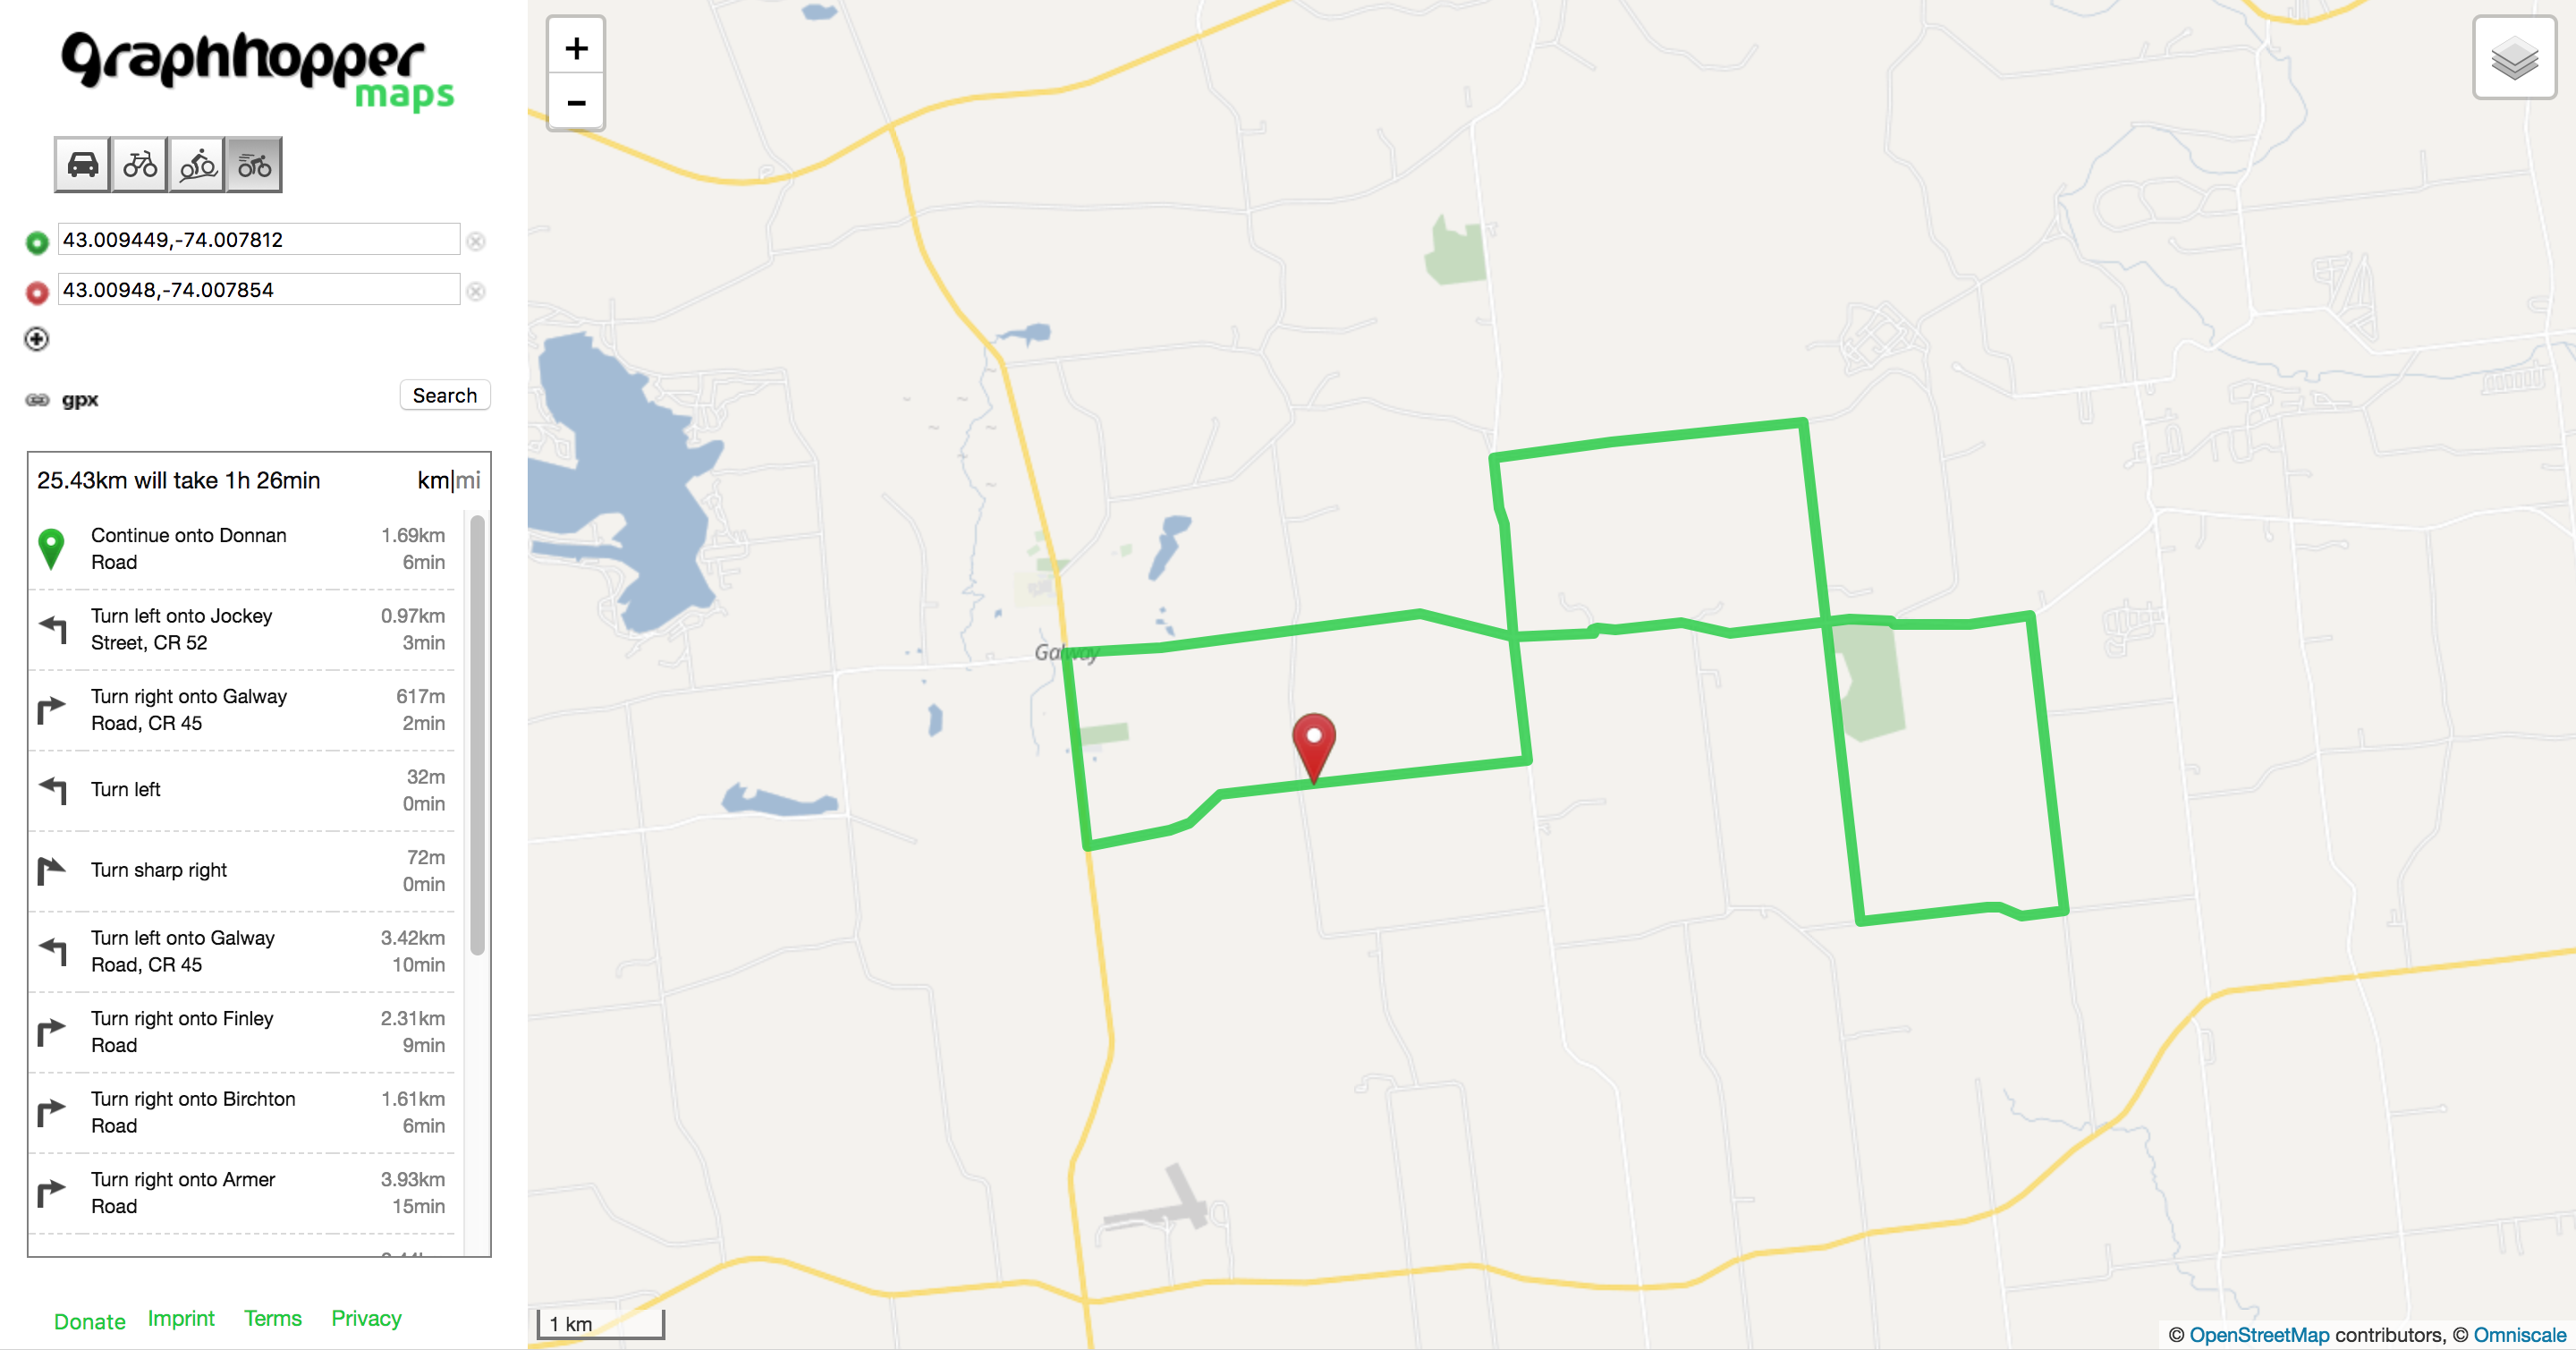
\includegraphics[width=\textwidth]{figs/vva-route}
    \end{center}
    \caption{Example route produced by our implementation of the VVA algorithm.}
    \label{fig:vva-example}
\end{figure}

\begin{figure}
    \begin{center}
        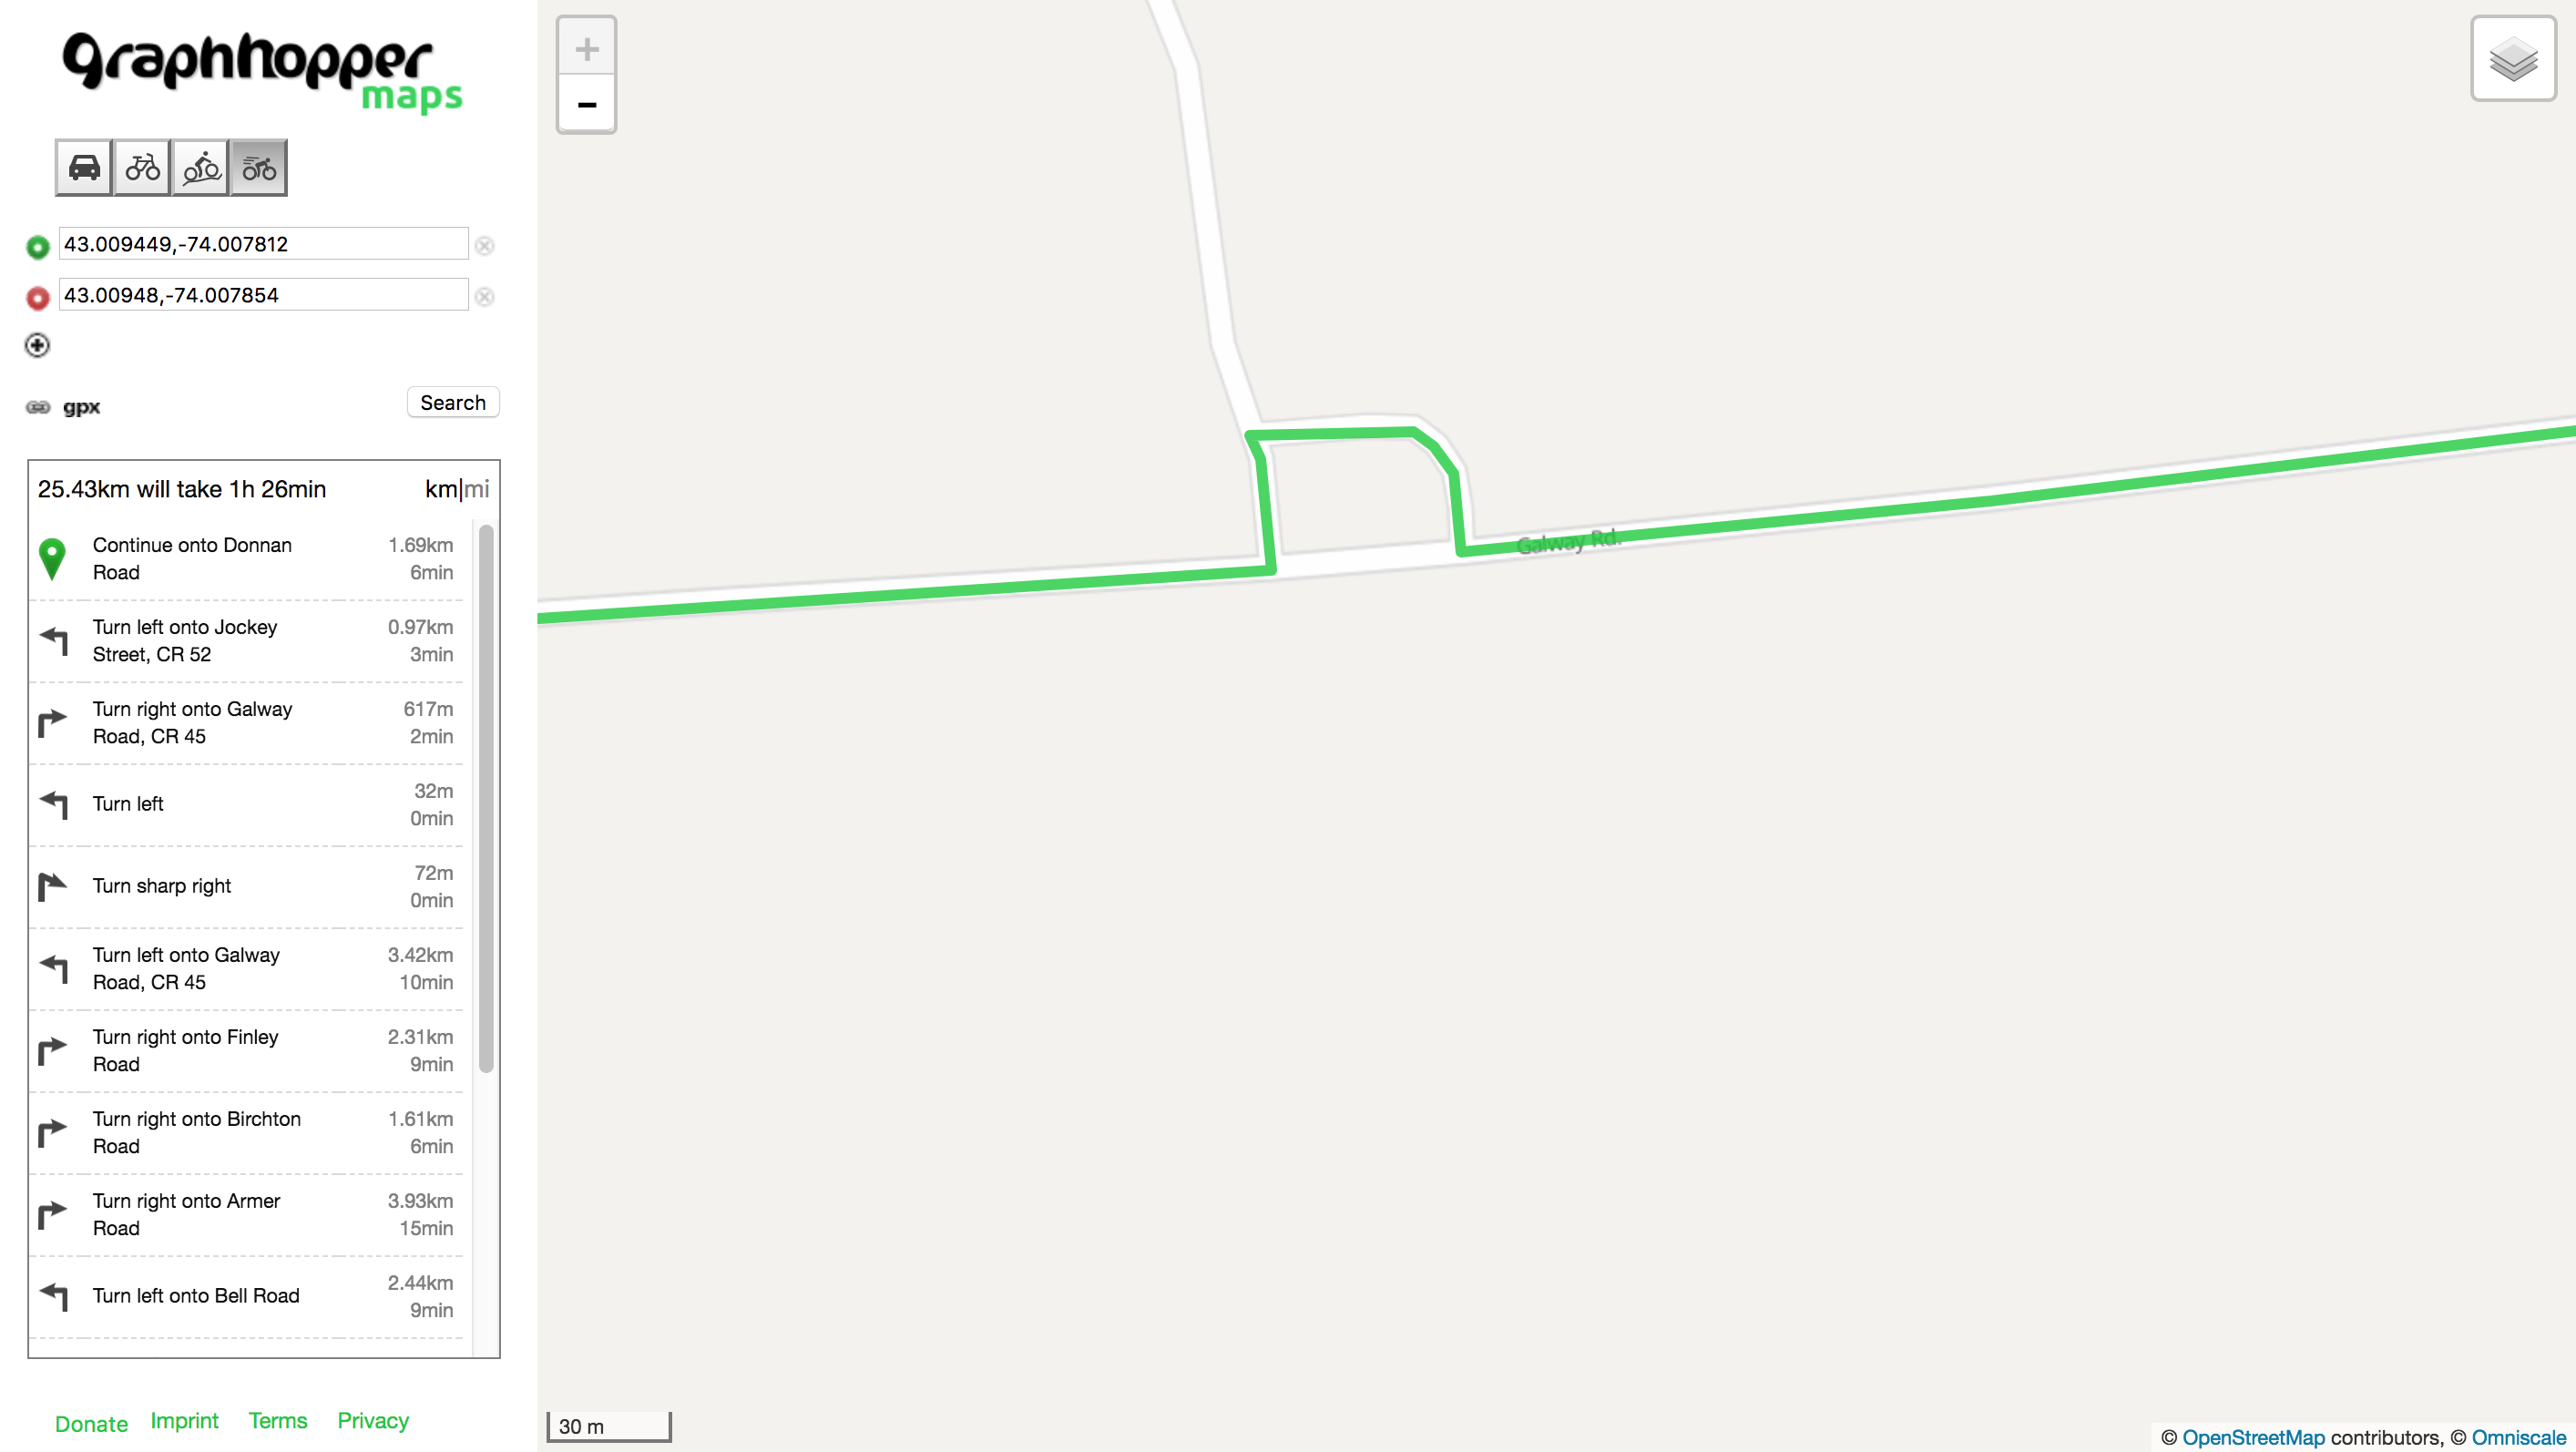
\includegraphics[width=\textwidth]{figs/vva-route-turn}
    \end{center}
    \caption{Quick turns in VVA example route. Inset in Figure \ref{fig:vva-example}}
    \label{fig:vva-example-turn}
\end{figure}


\subsubsection{LS Implementation}
Compared to the the VVA algorithm, the LS algorithm is more complex so our implementation differs more from the pseudocode provided by \citeauthor{lu2015arc}. There are many more implementation choices to be made. Recall that this algorithm works by connecting together attractive arcs with shortest paths known as ``blank path segments." 

Implicitly defined in the LS algorithm is an object which represents the solution built up through iterations. We call this object a ``Route" and provide a unified interface for adding and removing arcs from this path. When adding and removing arcs, internally the object maintains the blank path segment invariant by calculating shortest paths and storing these paths. When it is time to return return the actual path to GraphHopper, the Route object simply iterates over stored attractive arcs and shortest paths (blank path segments) in the correct order. Since we are using a contraction hierarchy shortest path algorithm to compute the blank path segments, we recursively ``unpack" any shortcuts (to get the original roads) before returning the solution to GraphHopper. 

Our Candidate Arc Set (CAS) computation also differs in the way we spatially fetch arcs. We do not use a grid index and fetch all arcs whose grids overlap with the pruning ellipse.  Instead, we perform a breath first search starting at our start node only continuing our search outward if a given road is inside of our pruning ellipse. When the search returns, we have a list of all arcs that are contained solely inside of the pruning ellipse. We compute CAS feasibility of these arcs using the same contraction hierarchy shortest path algorithm used to calculate blank path segments. Our scores and costs are identical to those used in our VVA implementation.

Because the LS algorithm is randomized, running the same query multiple times produces different routes. Figure \ref{fig:ls-route1} shows a perfectly circular route. However, a route with these characteristics is not always generated by the algorithm. Running the same query may produce a route such as Figure \ref{fig:ls-route2}. The route in Figure \ref{fig:ls-route2} contains two subpaths which extend outward and return on the same path like cul-de-sacs. In the most extreme case, shown in Figure \ref{fig:ls-route3}, the route is solely composed of these ``backtracking" subpaths. This results from the LS algorithm because attractive arc are being glued together by shortest paths; The shortest path back after taking an attractive arc may be the same path taken to get to the arc's start.

This backtracking shown in Figure \ref{fig:ls-routes} may be undesirable for cyclists. While riding on the same road more than once is not inherently undesirable for recreational cyclists, this may pose a safety issue. Following a route with excess backtracking requires numerous U-turns which can be dangerous for cyclists.  

\begin{figure}
\begin{subfigure}{.48\linewidth}
\centering
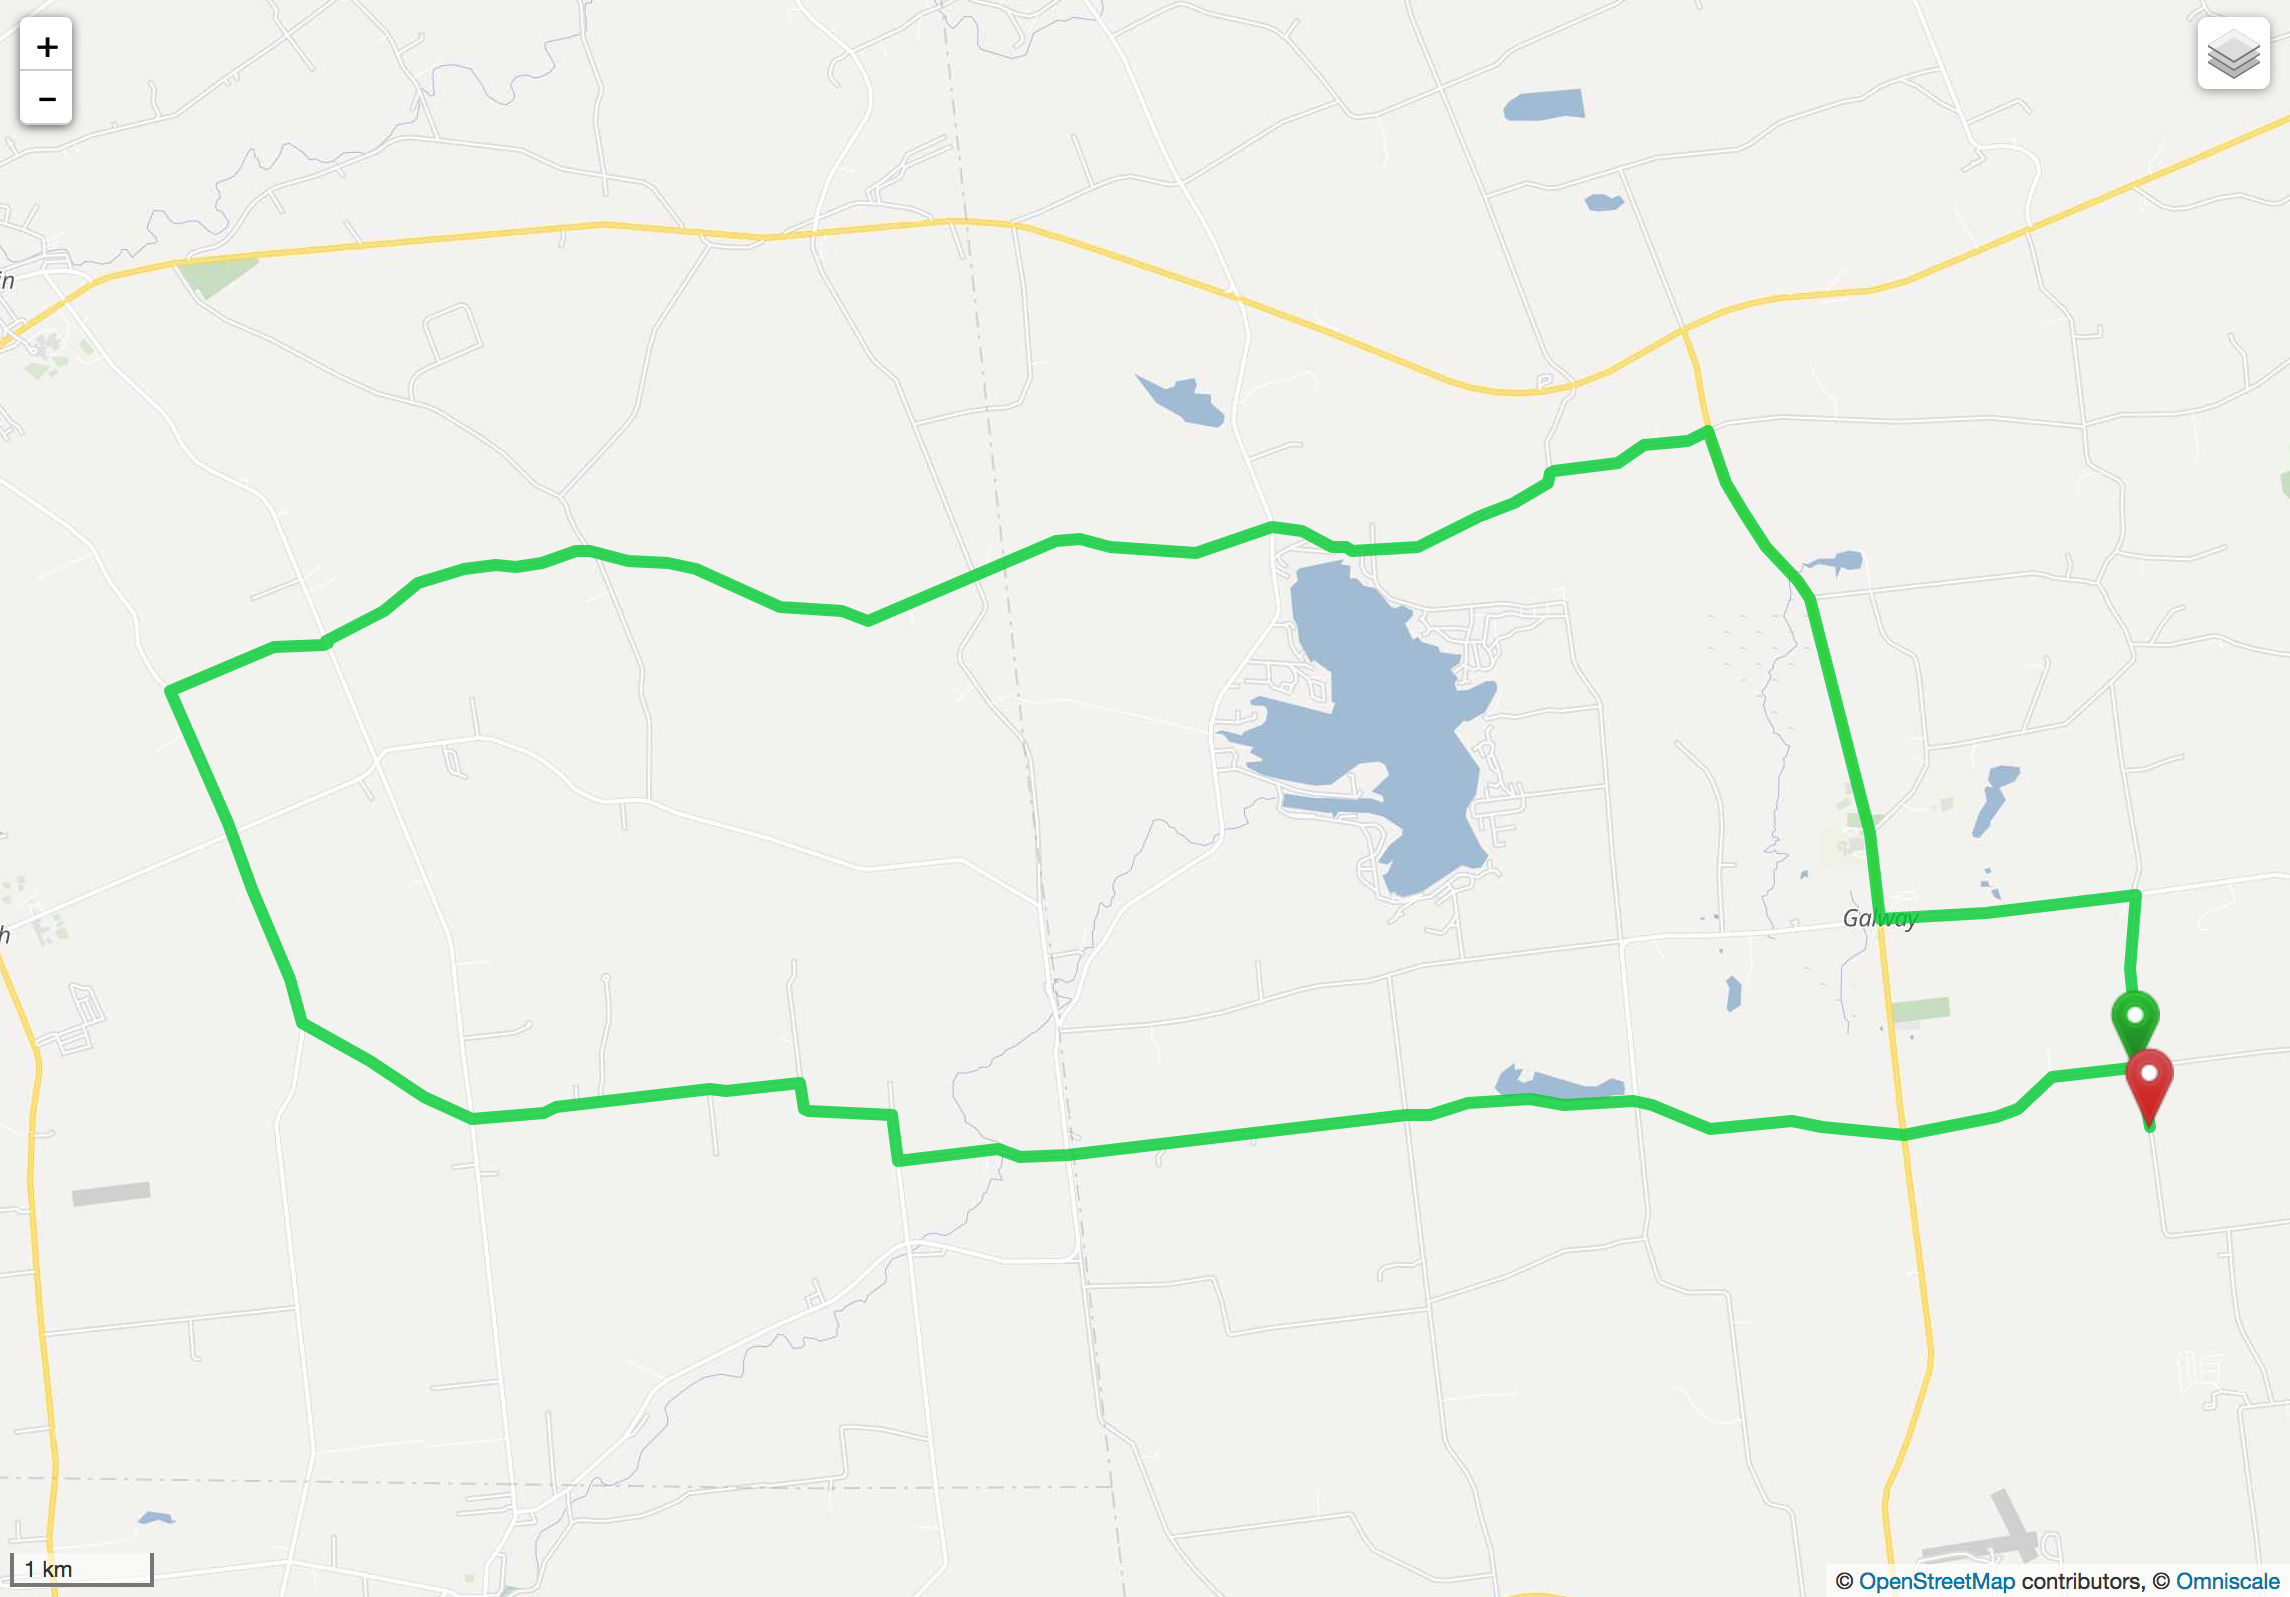
\includegraphics[width=\textwidth]{figs/ls-route1}
\caption{Perfectly circular route}
\label{fig:ls-route1}
\end{subfigure}%
\hfill
\begin{subfigure}{.48\linewidth}
\centering
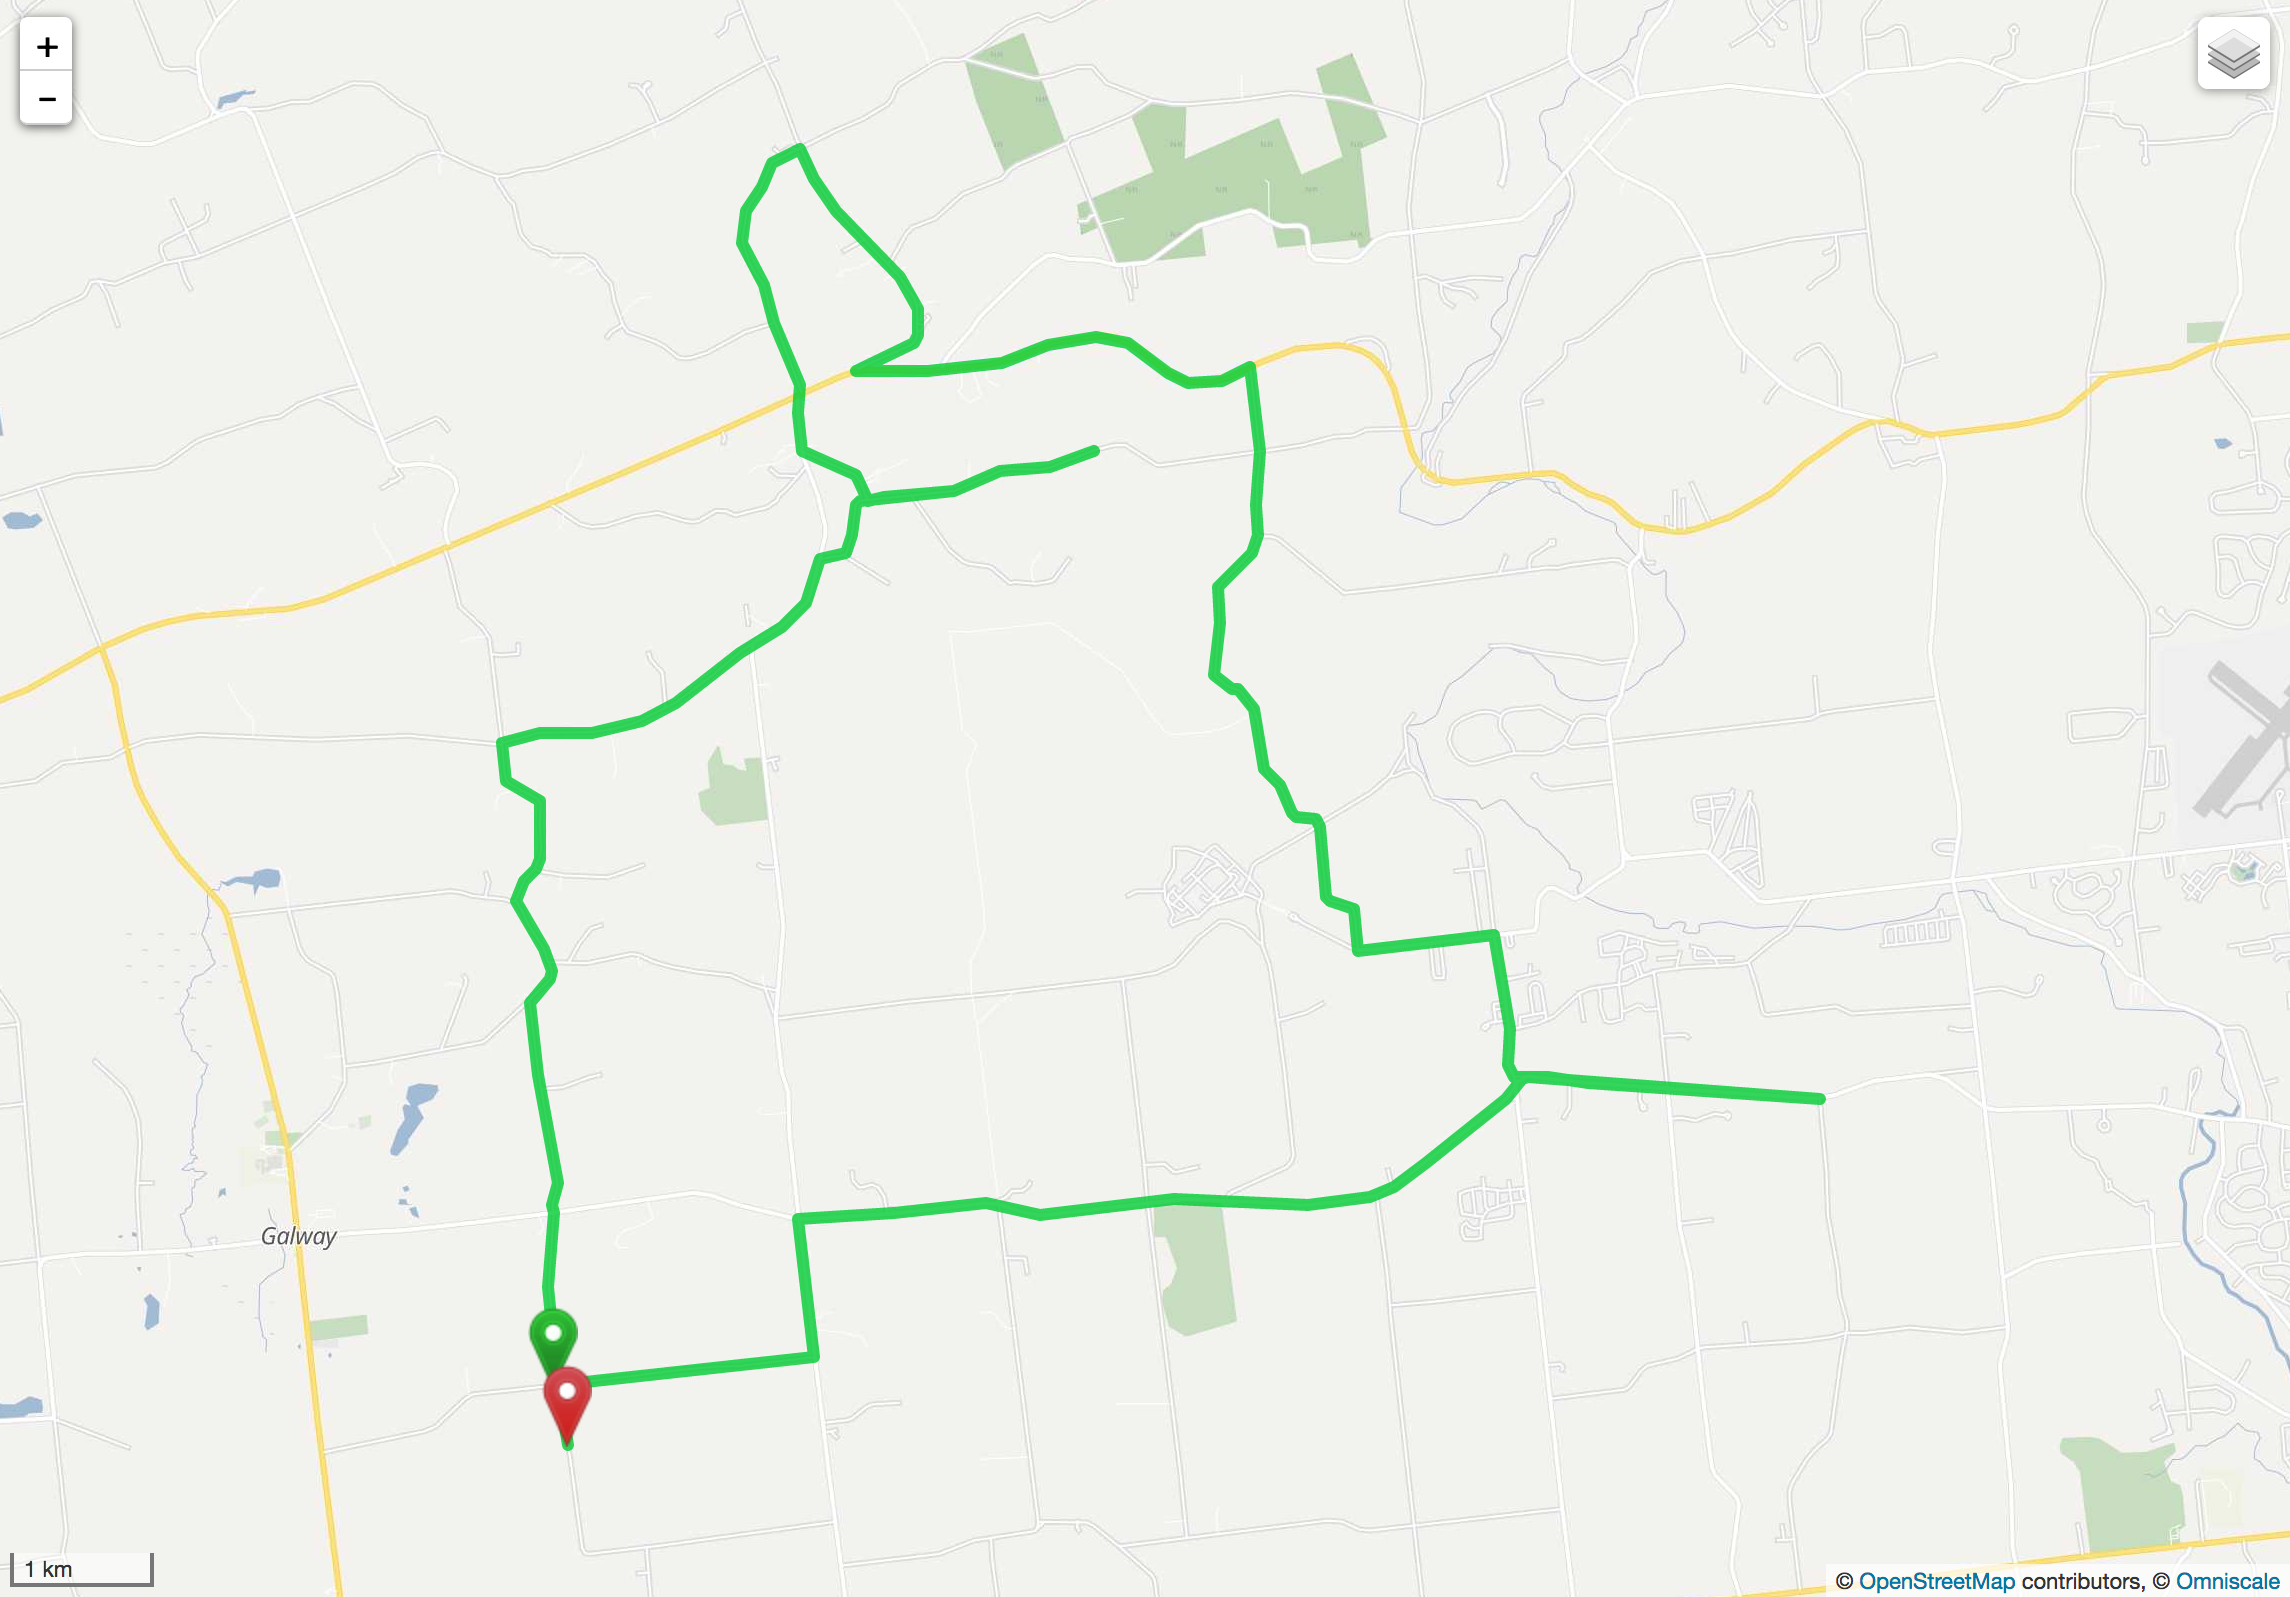
\includegraphics[width=\textwidth]{figs/ls-route2}
\caption{Route with some backtracking}
\label{fig:ls-route2}
\end{subfigure}\\[1ex]
\begin{center}
\begin{subfigure}{0.48\linewidth}
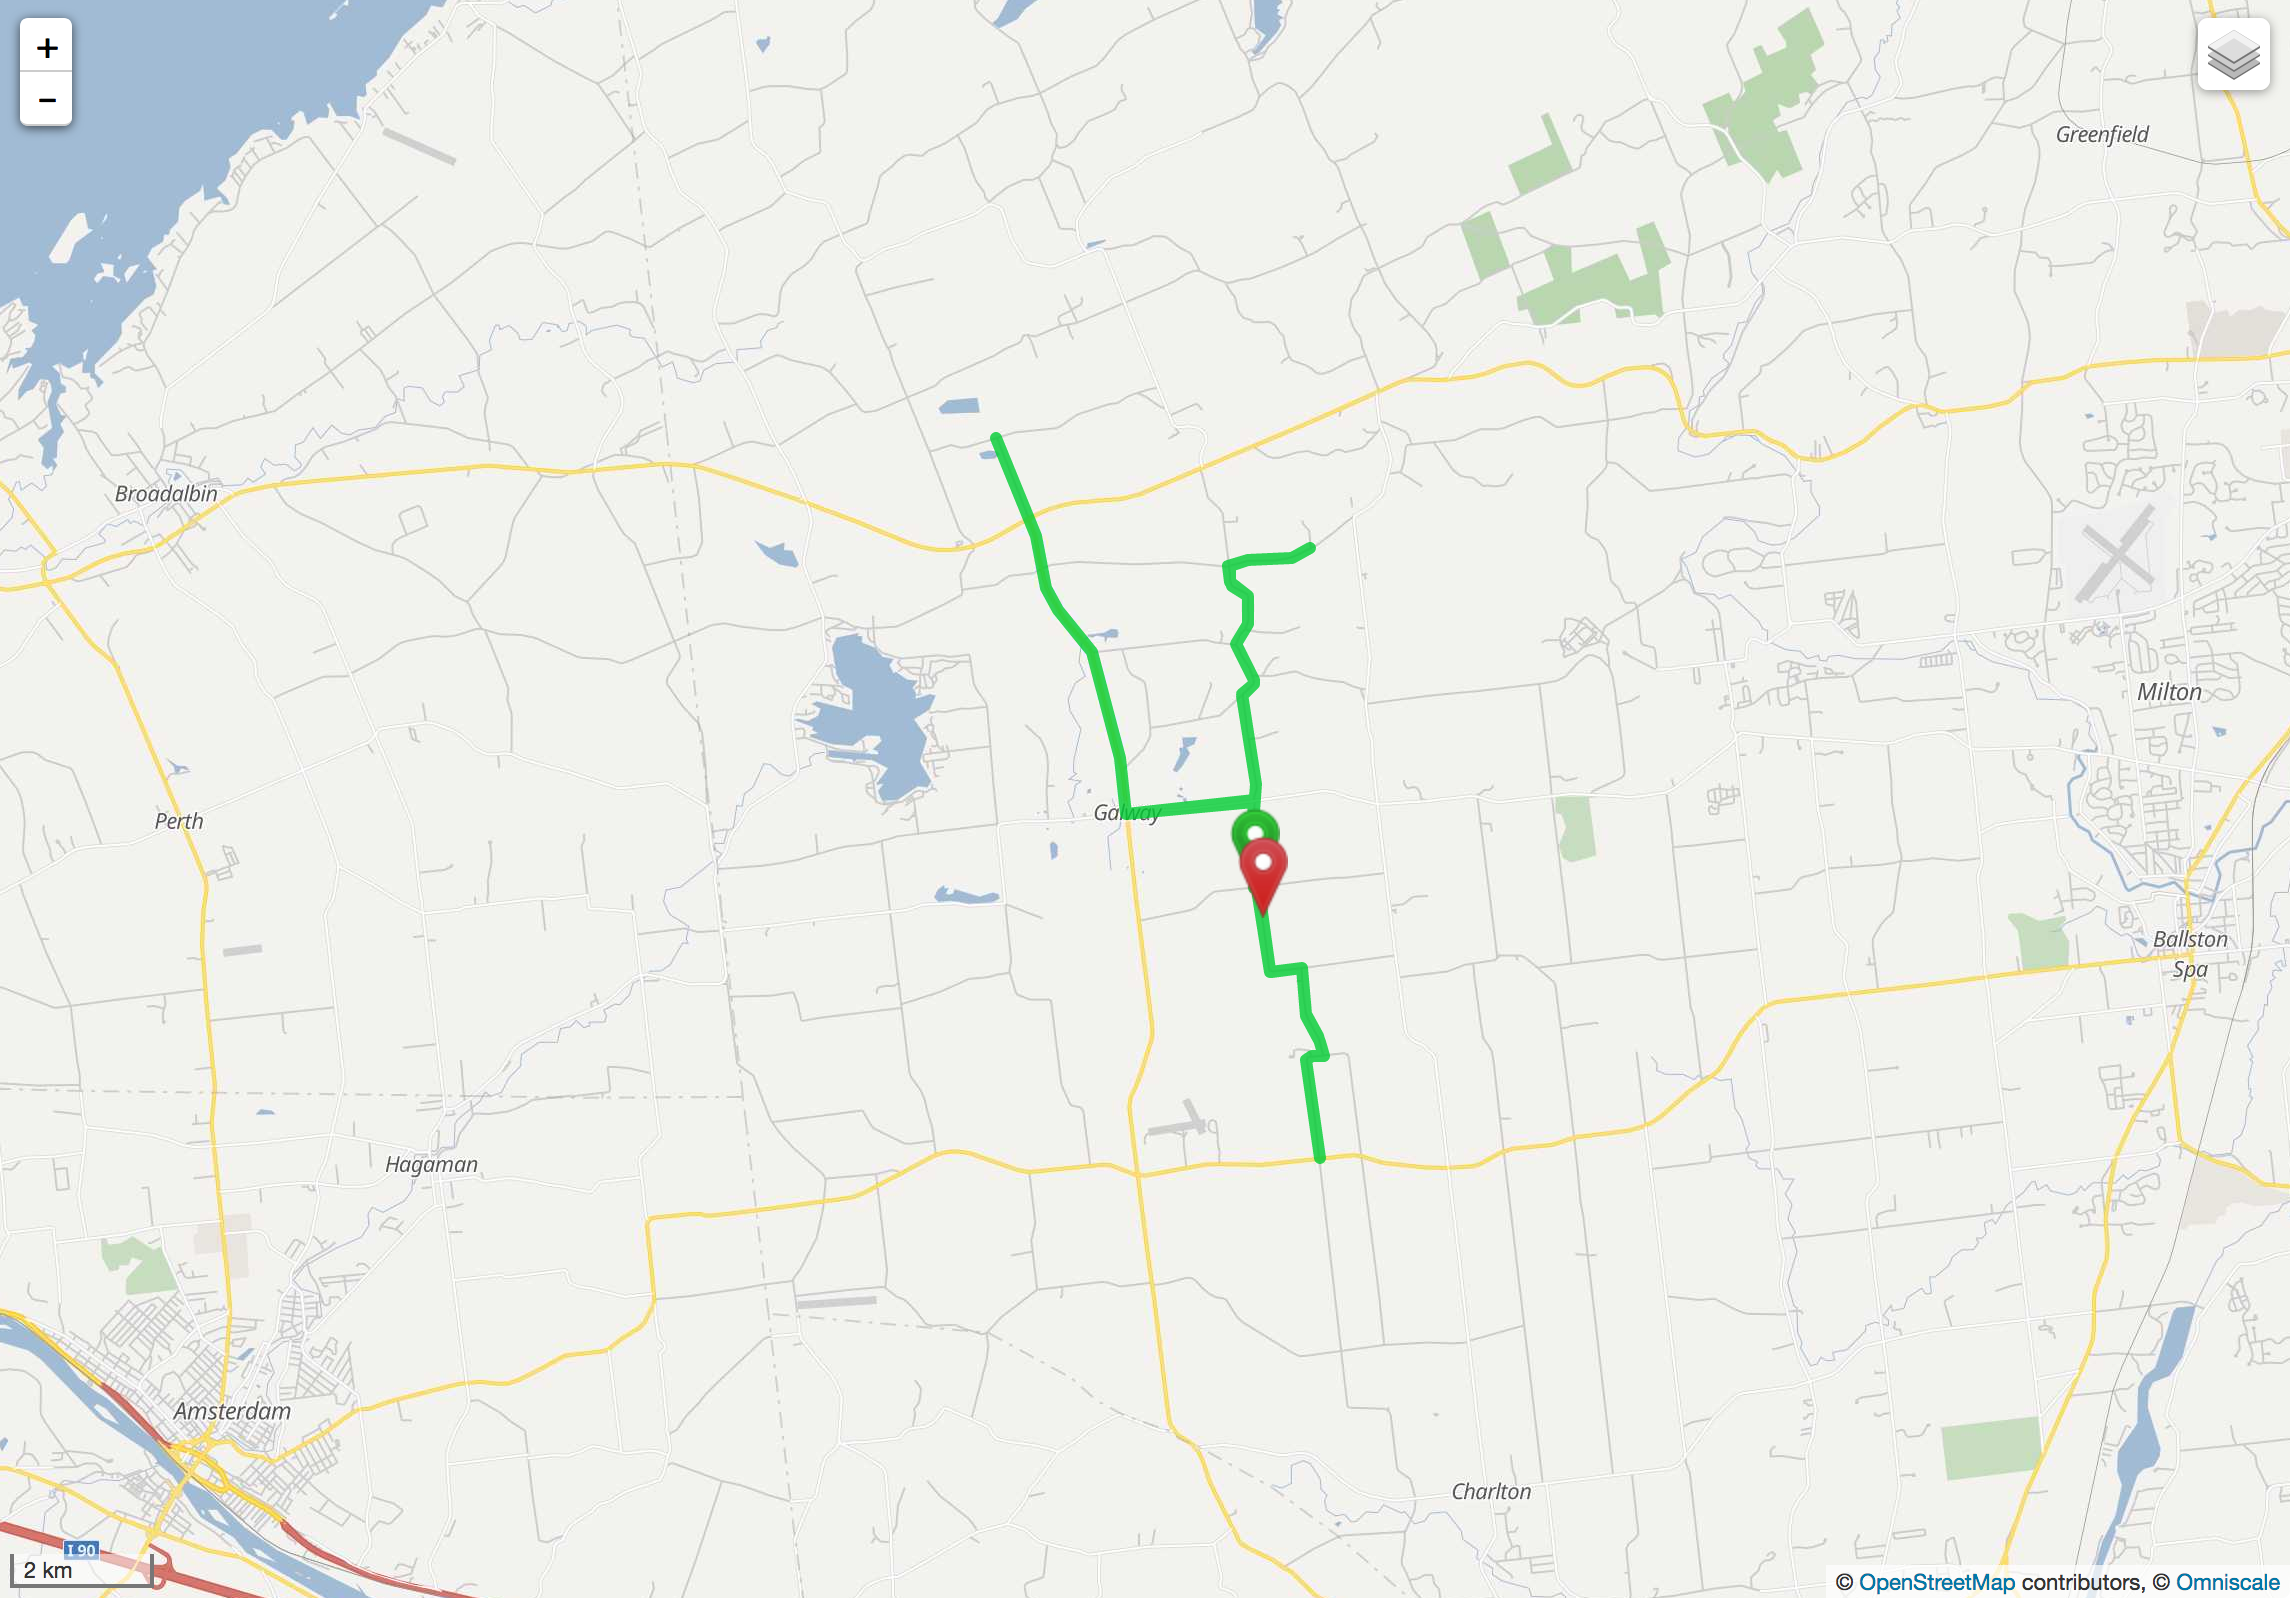
\includegraphics[width=\textwidth]{figs/ls-route3}
\caption{Route with excess backtracking}
\label{fig:ls-route3}
\end{subfigure}
\end{center}
\caption{Example routes generated by our LS implementation}
\label{fig:ls-routes}
\end{figure}

\subsection{Our LS Variants}
Our research implementing the LS algorithm in GraphHopper lead us to the following observations about the algorithm:
\begin{enumerate}
    \item LS does not avoid backtracking when creating blank path segments.
    \item LS tries to get as close to the cost budget as possible.
    \item LS puts very few restrictions on what is considered an attractive arc.
    \item LS does not penalize turns.
\end{enumerate}
We introduce a few variants of LS in order to address these observations.

\subsubsection{Budget Allowance}
$GeneratePath$ (Algorithm \ref{alg:ils-lu-genpath}) makes the greedy choice to insert a candidate arc at the smallest blank path segment in the route. This function continuously inserts candidate arcs until the CAS is empty or the cost budget is exhausted. This means that the path returned by Algorithm \ref{alg:ils-lu-genpath} will normally be very close to the maximum cost. 

The intuition is if the initial route generated by Algorithm \ref{alg:ils-lu-genpath} is very close to the budget, then there may not be enough budget remaining to make big changes to the route. Therefore, the ILS may get stuck in a local optimum. The ``budget allowance" variant aims to solve this by leaving more budget for later iterations of the search. Given a fixed percentage $0 < p < 1$, this variant ensures that Algorithm 6 is only allowed to use $p * RemainingBudget$ when constructing the path at any given iteration. 

\subsubsection{Incremental Budget}
The ``incremental budget" variant is similar to the ``budget allowance" variant and aims to solve the same problem. However, instead of using a fixed budget percentage, it a minimum budget percentage $p_{min}$. Over the course of the ILS iterations, the allowed budget scales from $p_{min}$ to $1$ in increments of $(1 - p_{min}) / iterations$. 

\subsubsection{Arc Restrictions}
This variant changes how arcs are chosen to be included in a CAS. In the baseline LS implementation, attractive arcs are arcs whose score is greater than zero. This variant takes in two parameters $min\_road\_length$ and $min\_road\_score$. An arc is only considered attractive and added to the CAS if its distance in meters is greater than $min\_road\_length$ and its score is greater than $min\_road\_score$. The intuition behind these restrictions is that the algorithm should not route to an attractive arc that is very small and have a meager score. Similarly, for a particular arc, the distance spent to traverse it should be worthwhile and this is generally true of longer arcs with higher scores. 

\subsubsection{No Backtracking}
This variant attempts to solve the issue displayed in Figure \ref{fig:ls-routes} by ``blacklisting" roads from the shortest path computations. As the algorithm builds up intermediate solutions, we keep track of all the arcs currently in the solution using a HashSet. When it is time to calculate a blank path segment to an attractive arc, we restrict which arcs are allowed to be traversed by the shortest path algorithm using the HashSet and the attractive arc. When calculating the blank path segment away from the attractive arc, we need to blacklist not only the roads in the solution but the roads in the first blank path segment as well. This practice has two key implementation details which we address.

First, blacklisting roads may break the shortest path computation. In a connected graph there is always some shortest path between any two nodes. However, if we restrict which roads are allowed in the search then it is possible that we may have no shortest path. For example, consider an attractive arc at the end of a dead end road. Computing the first blank path segment to the arc will succeed but we cannot take the same path back so we have no return segment. In the case where we have no available blank path segment, we set the total path cost to \emph{infinity}. This means that the arc will no longer be included in the CAS since it cannot feasibly update any arcs. 

Second, this blacklisting process does not work well with contraction hierarchies. Recall that a contraction-hierarchy shortest-path algorithm traverses over contracted ``shortcut" edges in the graph. The actual returned shortest path is recreated by finding the original roads which these shortcuts skip over. When determining if a road is blacklisted in our shortest path traversal, we need to check whether our current road is a shortcut and if it is, make sure none of the roads it skips are also blacklisted. This is quite challenging since a shortcut may skip multiple roads and may skip other shortcut edges. This means that we need to recursively ``unpack" a shortcut (and any skipped shortcuts)  before we can determine if we should avoid the arc. This is effectively undoing all the pre-computation that is done when the contraction hierarchy is initialized. In order to avoid this problem, our no-backtracking variant does not use a contraction hierarchy shortest-path algorithm.


\section{Evaluation}
We ran a series of experiments in order to evaluate the performance of the VVA algorithm, the LS algorithm, and our LS variants. 

\subsection{Data Collection}
%Our data set is the OpenStreetMap file

\subsection{Experimental Results}

\subsubsection{Unit Scoring}
\subsubsection{Scaled Scoring}

\subsection{Integer Programming}
\citeauthor{verbeeck2014extension} show that it is possible to model the AOP using Integer Programming.

\section{Future Work}

\section{Conclusions}

\FloatBarrier
\bibliographystyle{plainnat}
\bibliography{references}

\end{document}
